\documentclass[12pt,a4paper]{article}

\usepackage[a4paper,margin=1in]{geometry}
\usepackage{graphicx}
\usepackage{booktabs}
\usepackage{amsmath,amssymb}
\usepackage{float}
\usepackage{hyperref}
\usepackage{xcolor}
\usepackage{listings}
\usepackage{enumitem}
\usepackage{fancyhdr}
\usepackage{longtable}

\hypersetup{colorlinks=true,linkcolor=blue,urlcolor=blue}

\pagestyle{fancy}
\fancyhf{}
\lhead{ICS1512}
\rhead{Machine Learning Algorithms Laboratory}
\cfoot{\thepage}

\lstset{
language=Python,
basicstyle=\ttfamily\small,
numbers=left,
frame=single,
breaklines=true,
showstringspaces=false
}

\begin{document}

\begin{tabular}{|p{4cm}|p{11cm}|}
\hline
Experiment No. & 3 \\ \hline
Experiment Title & Regression Analysis using Linear and Regularized Models \footnote{\textbf{GitHub Repository: }\url{https://github.com/Kavin-ks/Machine-Learning-Projects}}\\ \hline
Student Name & Kavinsoorya K S \\ \hline
Register Number & 3122247001030 \\ \hline
Faculty & Dr. Poreddy Ajay Kumar Reddy \\ \hline
Submission Date & July 25, 2026 \\ \hline
\end{tabular}

\vspace{0.5cm}

\section{Objective}
The objective of this experiment is to implement linear and regularized regression models for predicting a continuous target variable, evaluate their performance using multiple metrics, visualize model behavior, and analyze overfitting, underfitting, and bias--variance characteristics.

\section{Problem Statement}
In continuous predictive modeling, financial institutions require accurate estimation of loan sanction amounts based on applicant demographics, income stability, existing liabilities, and asset valuations. Mathematically, given a training dataset $\mathcal{D} = \{(\mathbf{x}_i, y_i)\}_{i=1}^n$ where $\mathbf{x}_i \in \mathbb{R}^d$ represents a $d$-dimensional vector of applicant attributes and $y_i \in \mathbb{R}$ represents the continuous target variable \textbf{Loan Sanction Amount (USD)}, the objective is to learn a hypothesis function $f(\mathbf{x}) = \mathbf{x}^T \boldsymbol{\beta}$ that minimizes prediction loss over unseen test instances while preventing overfitting caused by feature collinearity.

\section{Dataset Description}
The experiment is conducted using the Kaggle \textbf{Predict Loan Amount Dataset}. The dataset characteristics and train-test partitioning details are summarized in Table~\ref{tab:dataset_summary}.

\begin{longtable}{|p{6cm}|p{8cm}|}
\hline
Dataset Name & Predict Loan Amount Dataset \\ \hline
Dataset Source & Kaggle Repository \\ \hline
Initial Sample Size & 30,000 application records \\ \hline
Cleaned Sample Size (Valid Target) & 29,660 records (340 missing target rows dropped) \\ \hline
Total Raw Feature Count & 23 (12 numerical, 11 categorical) \\ \hline
Engineered Features (Post One-Hot) & 46 standardized numeric features \\ \hline
Target Attribute & Loan Sanction Amount (USD) \\ \hline
Missing Value Handling & Median (Numerical) / Mode (Categorical) \\ \hline
Train-Test Split Ratio & 80\% Training (23,728) / 20\% Testing (5,932) \\ \hline
\end{longtable}

Numerical attributes include \texttt{Age}, \texttt{Income (USD)}, \texttt{Loan Amount Request (USD)}, \texttt{Current Loan Expenses (USD)}, \texttt{Dependents}, \texttt{Credit Score}, \texttt{No. of Defaults}, \texttt{Property Age}, and \texttt{Property Price}. Categorical features include \texttt{Gender}, \texttt{Income Stability}, \texttt{Profession}, \texttt{Type of Employment}, \texttt{Location}, and active credit status flags.

\section{Exploratory Data Analysis}
Exploratory Data Analysis (EDA) was performed to understand feature distributions, target characteristics, missingness, and pairwise attribute relationships.

\subsection{Missing Value Heatmap}

\begin{figure}[H]
\centering
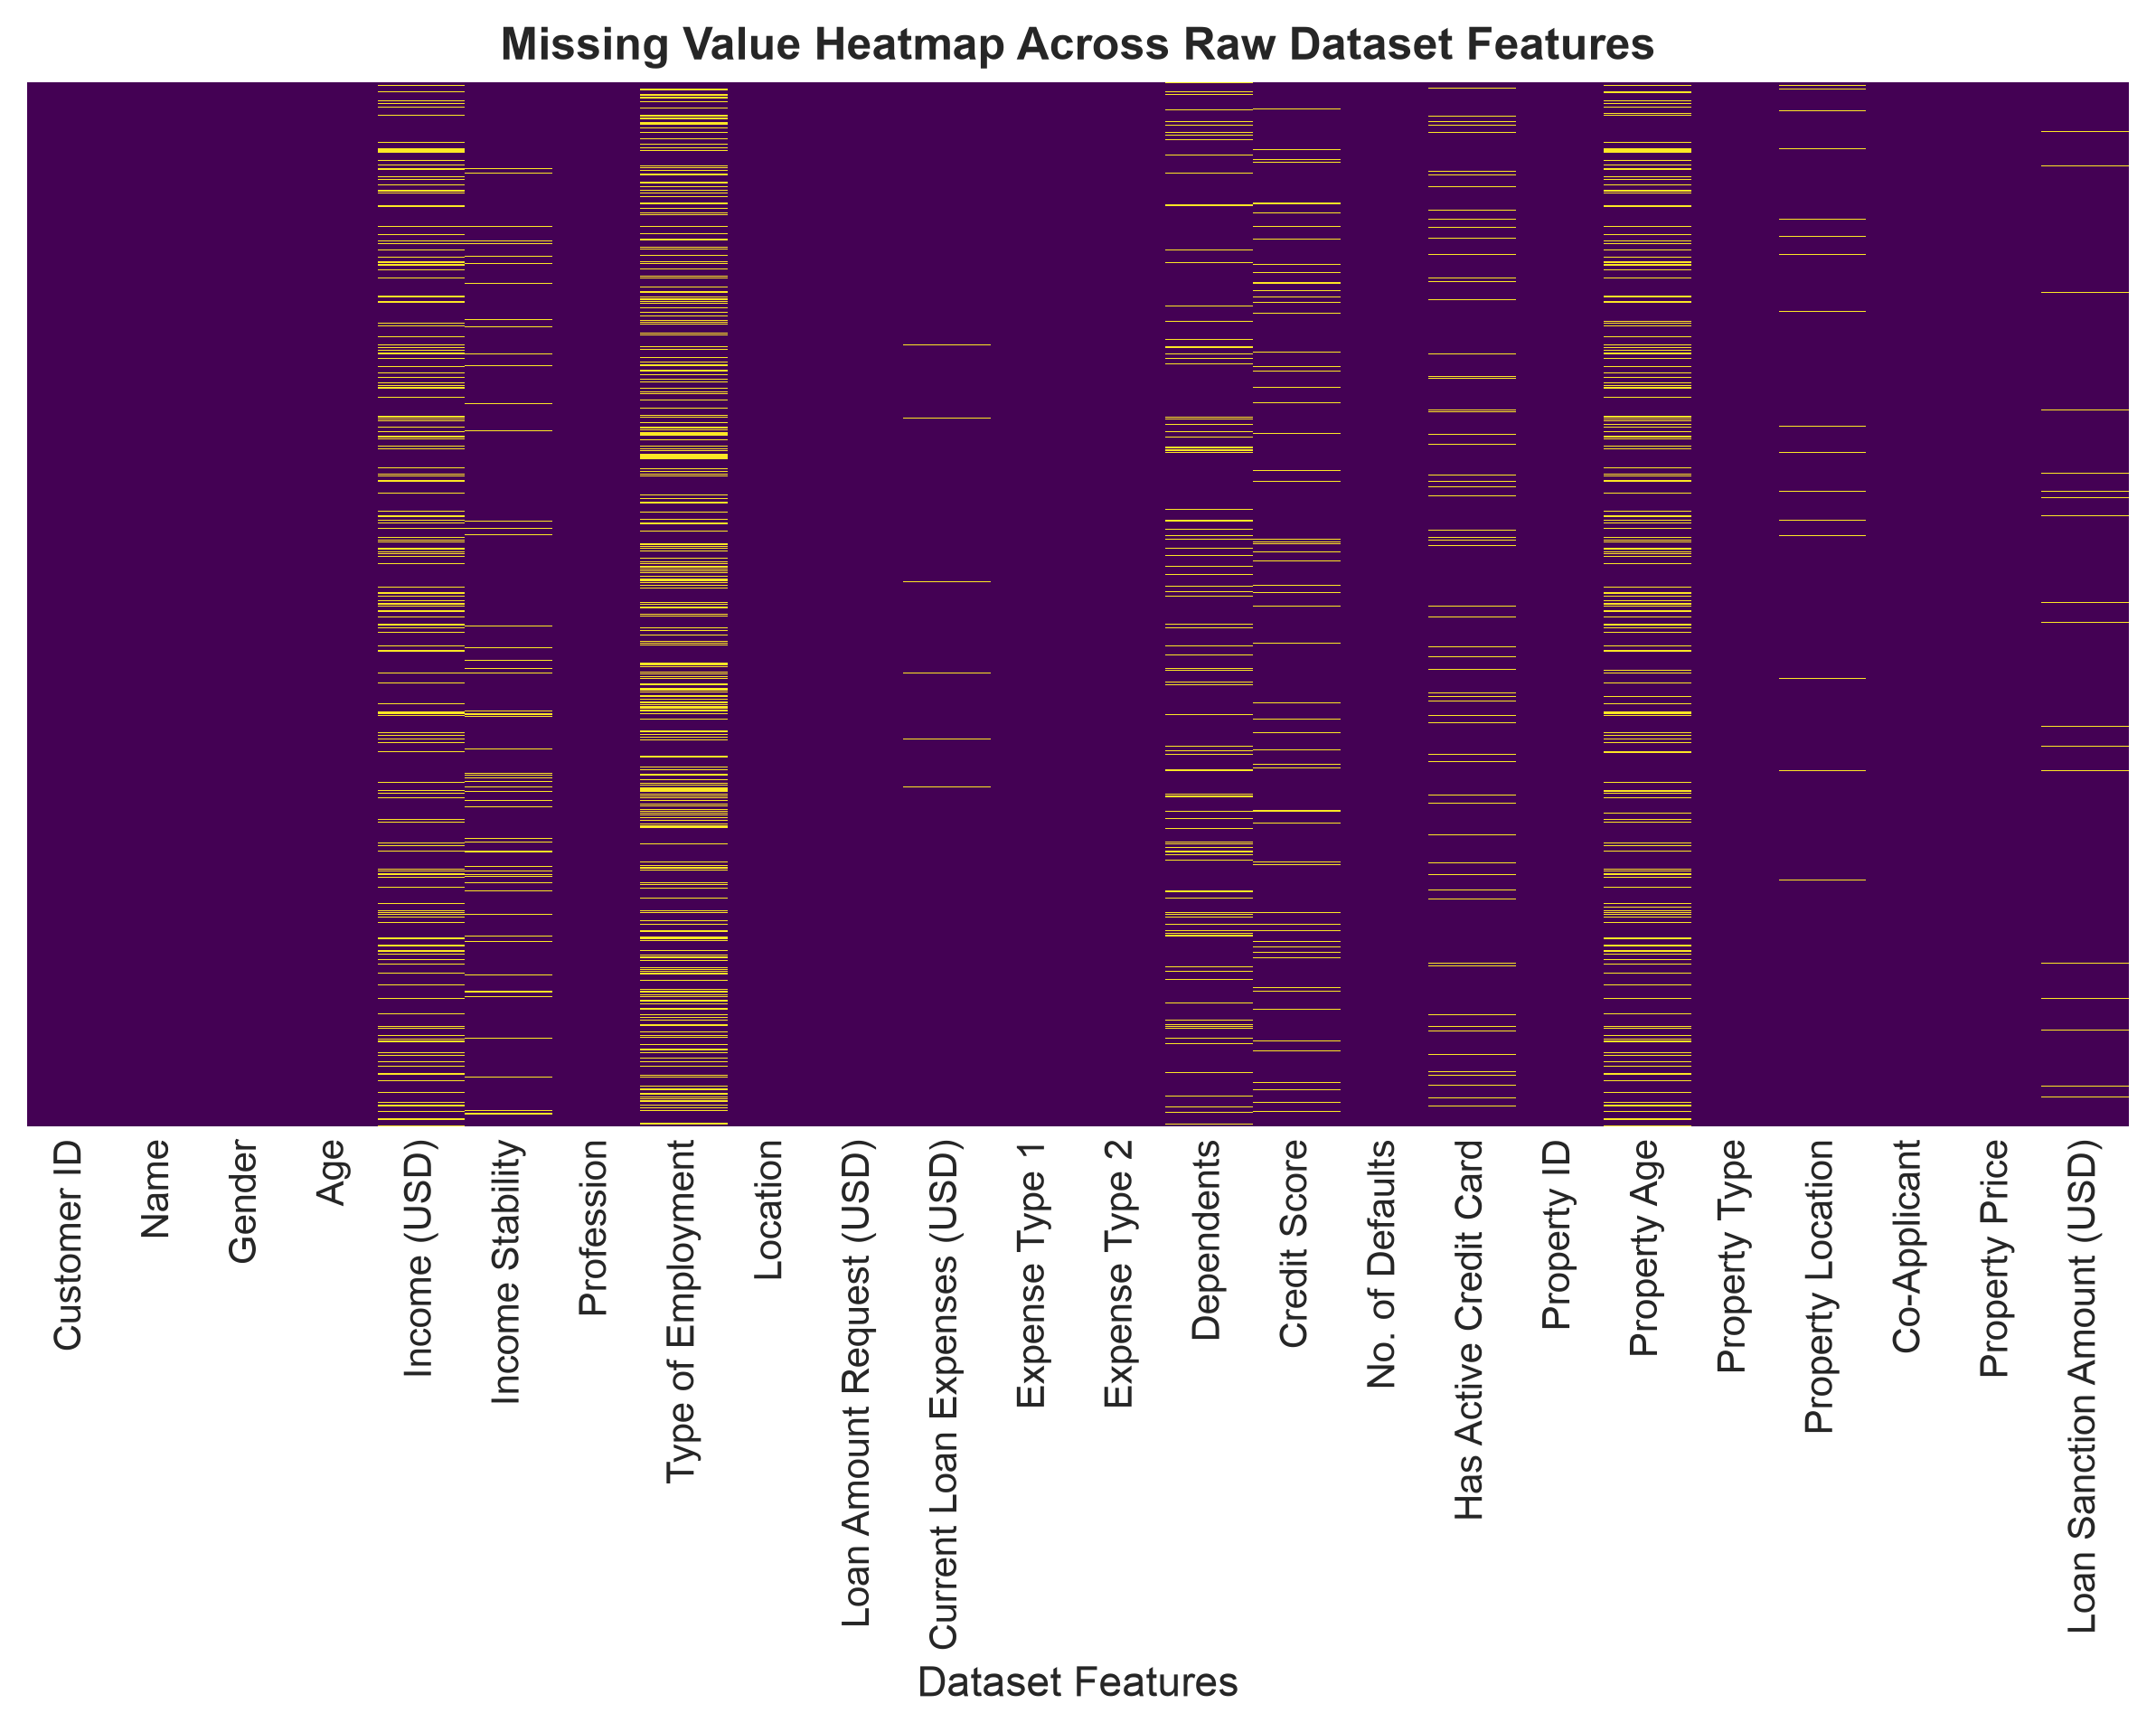
\includegraphics[width=0.8\linewidth]{images/missing_value_heatmap.png}
\caption{Missing Value Heatmap Across Raw Dataset Features}
\label{fig:missing_heatmap}
\end{figure}

\textbf{Inference:}
The missing value heatmap illustrates the distribution of missing entries across raw attributes before preprocessing. Notable missingness is observed in \texttt{Type of Employment} (7,270 missing), \texttt{Property Age} (4,850 missing), \texttt{Income (USD)} (4,576 missing), and \texttt{Dependents} (2,493 missing). This confirms the necessity of column-wise median and mode imputation.

\subsection{Target Variable Distribution}

\begin{figure}[H]
\centering
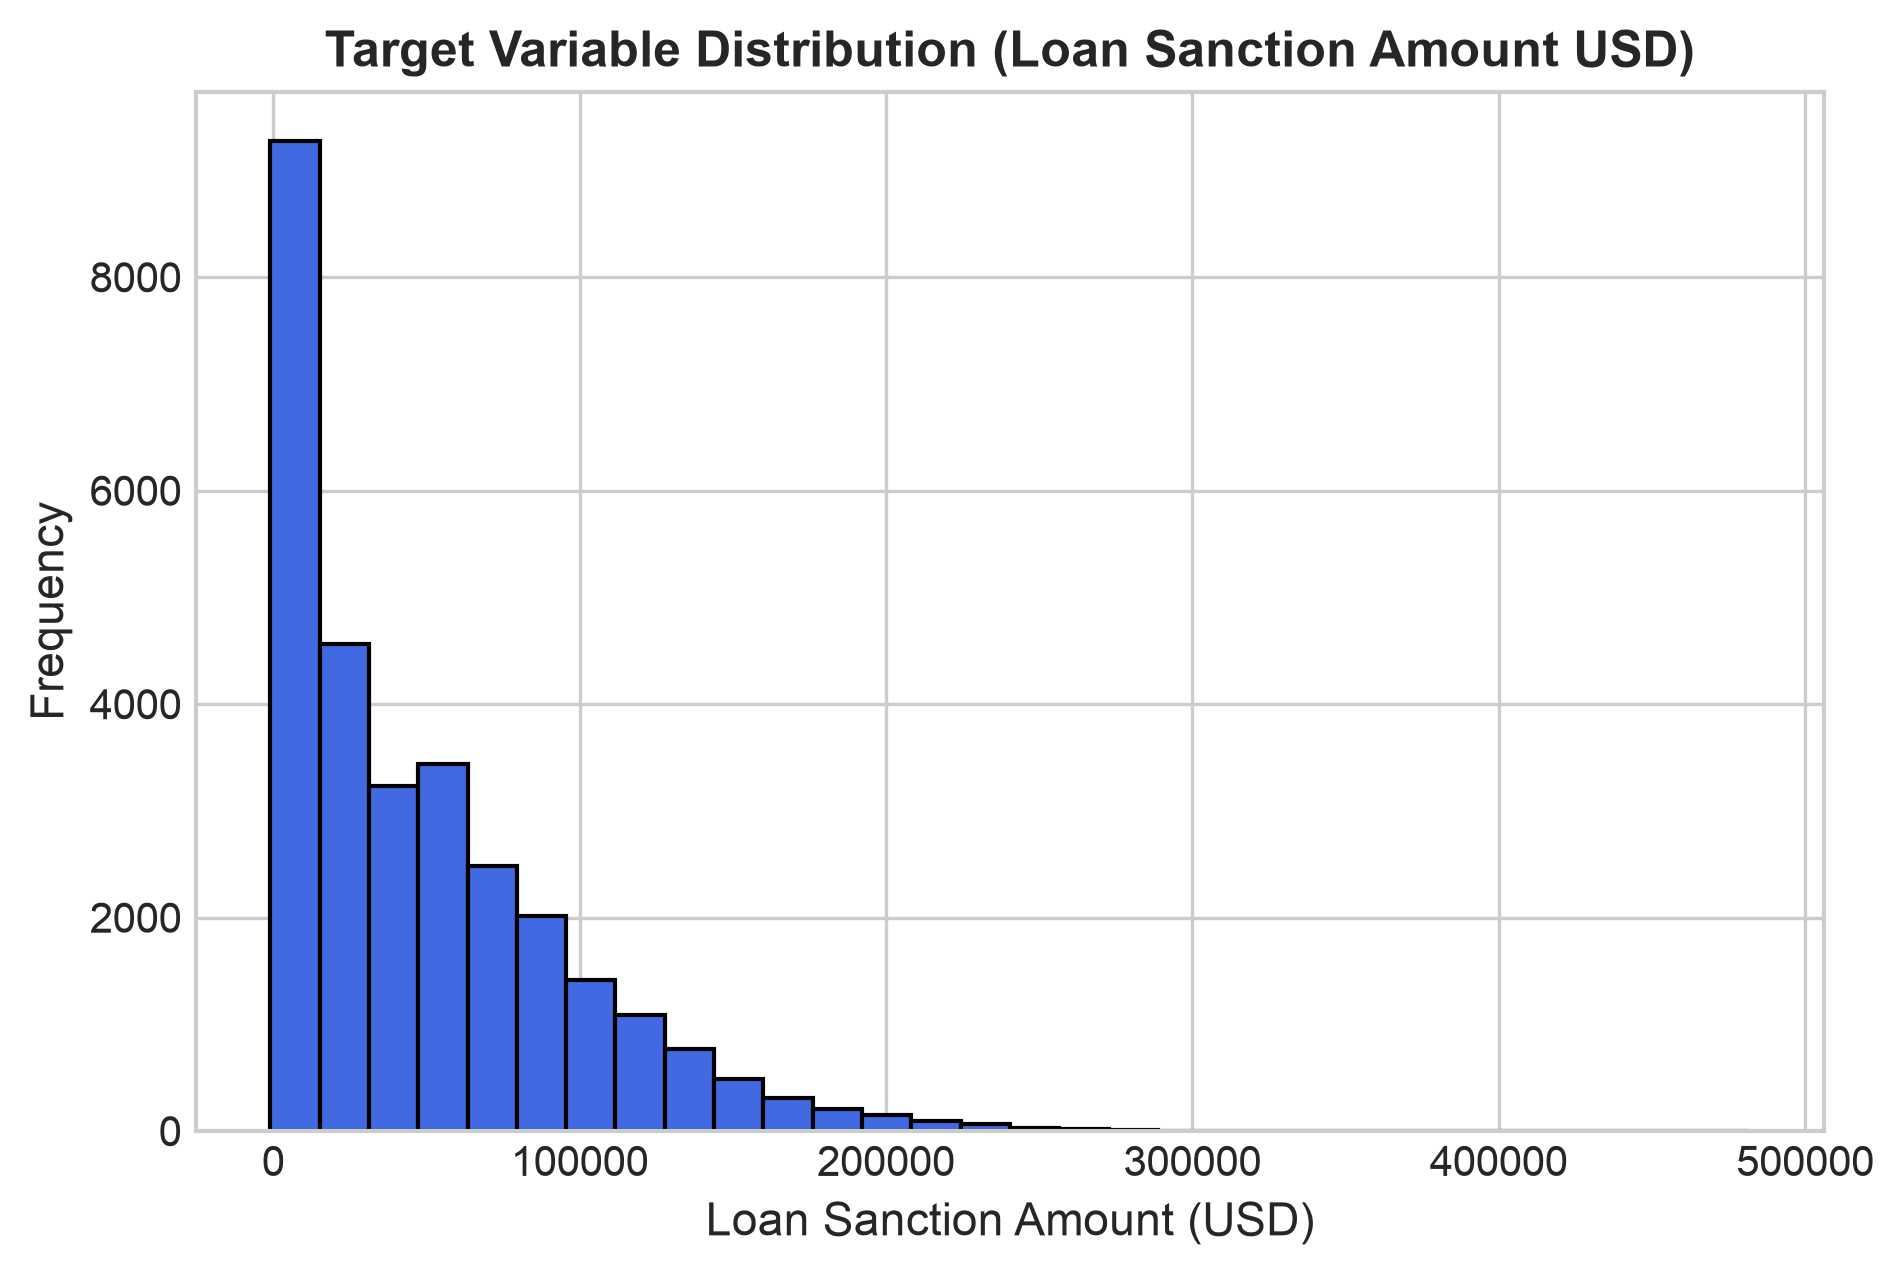
\includegraphics[width=0.7\linewidth]{images/target_distribution.png}
\caption{Distribution of Target Variable (Loan Sanction Amount USD)}
\label{fig:target_dist}
\end{figure}

\textbf{Inference:}
The target variable histogram reveals a positive right-skewed distribution. Most loan sanction amounts range between \$0 and \$100,000, with a median of \$35,209.40 and a maximum value reaching \$481,907.32. This skewness highlights the necessity of feature scaling prior to fitting regularized regression models.

\subsection{Feature Distributions}

\begin{figure}[H]
\centering
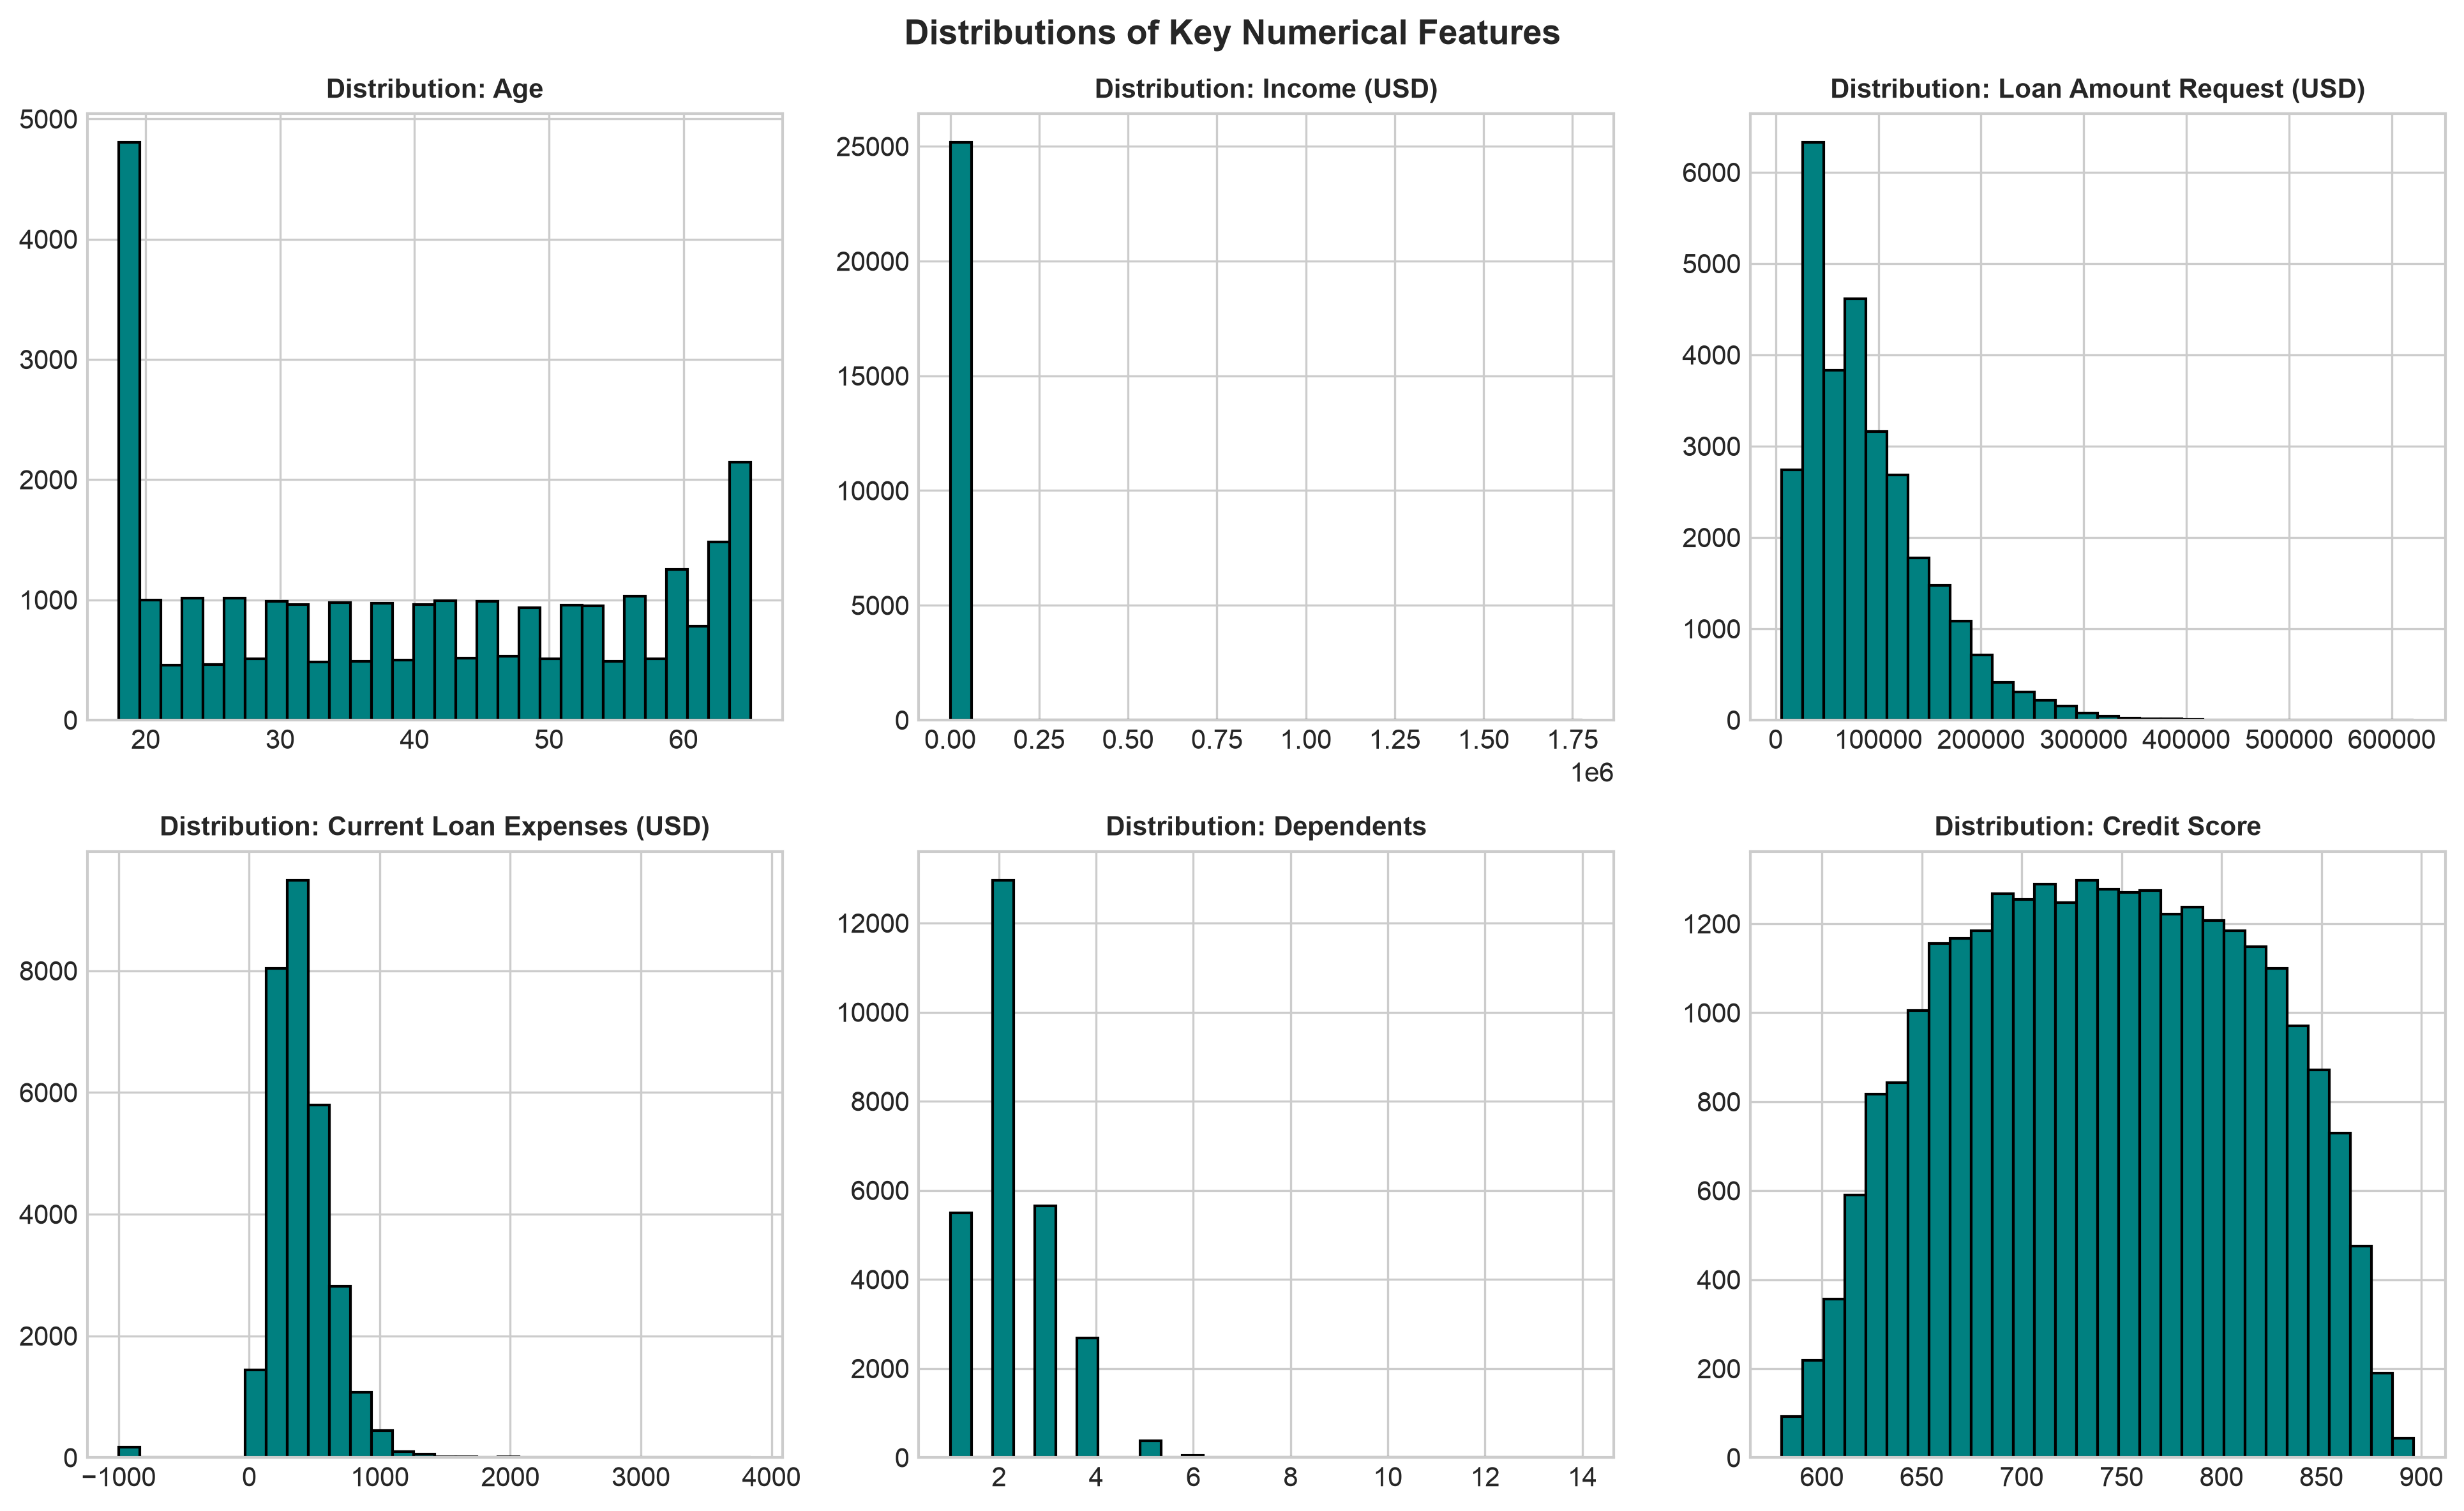
\includegraphics[width=0.85\linewidth]{images/feature_distribution.png}
\caption{Distributions of Key Numerical Features}
\label{fig:feat_dist}
\end{figure}

\textbf{Inference:}
Distributions of numerical predictors indicate that attributes like \texttt{Income (USD)} and \texttt{Property Price} are heavily right-skewed, whereas \texttt{Age} and \texttt{Credit Score} display near-uniform and normal distributions respectively. Standardizing all continuous variables to zero mean and unit variance ensures robust convergence.

\subsection{Pairwise Feature Correlation Matrix}

\begin{figure}[H]
\centering
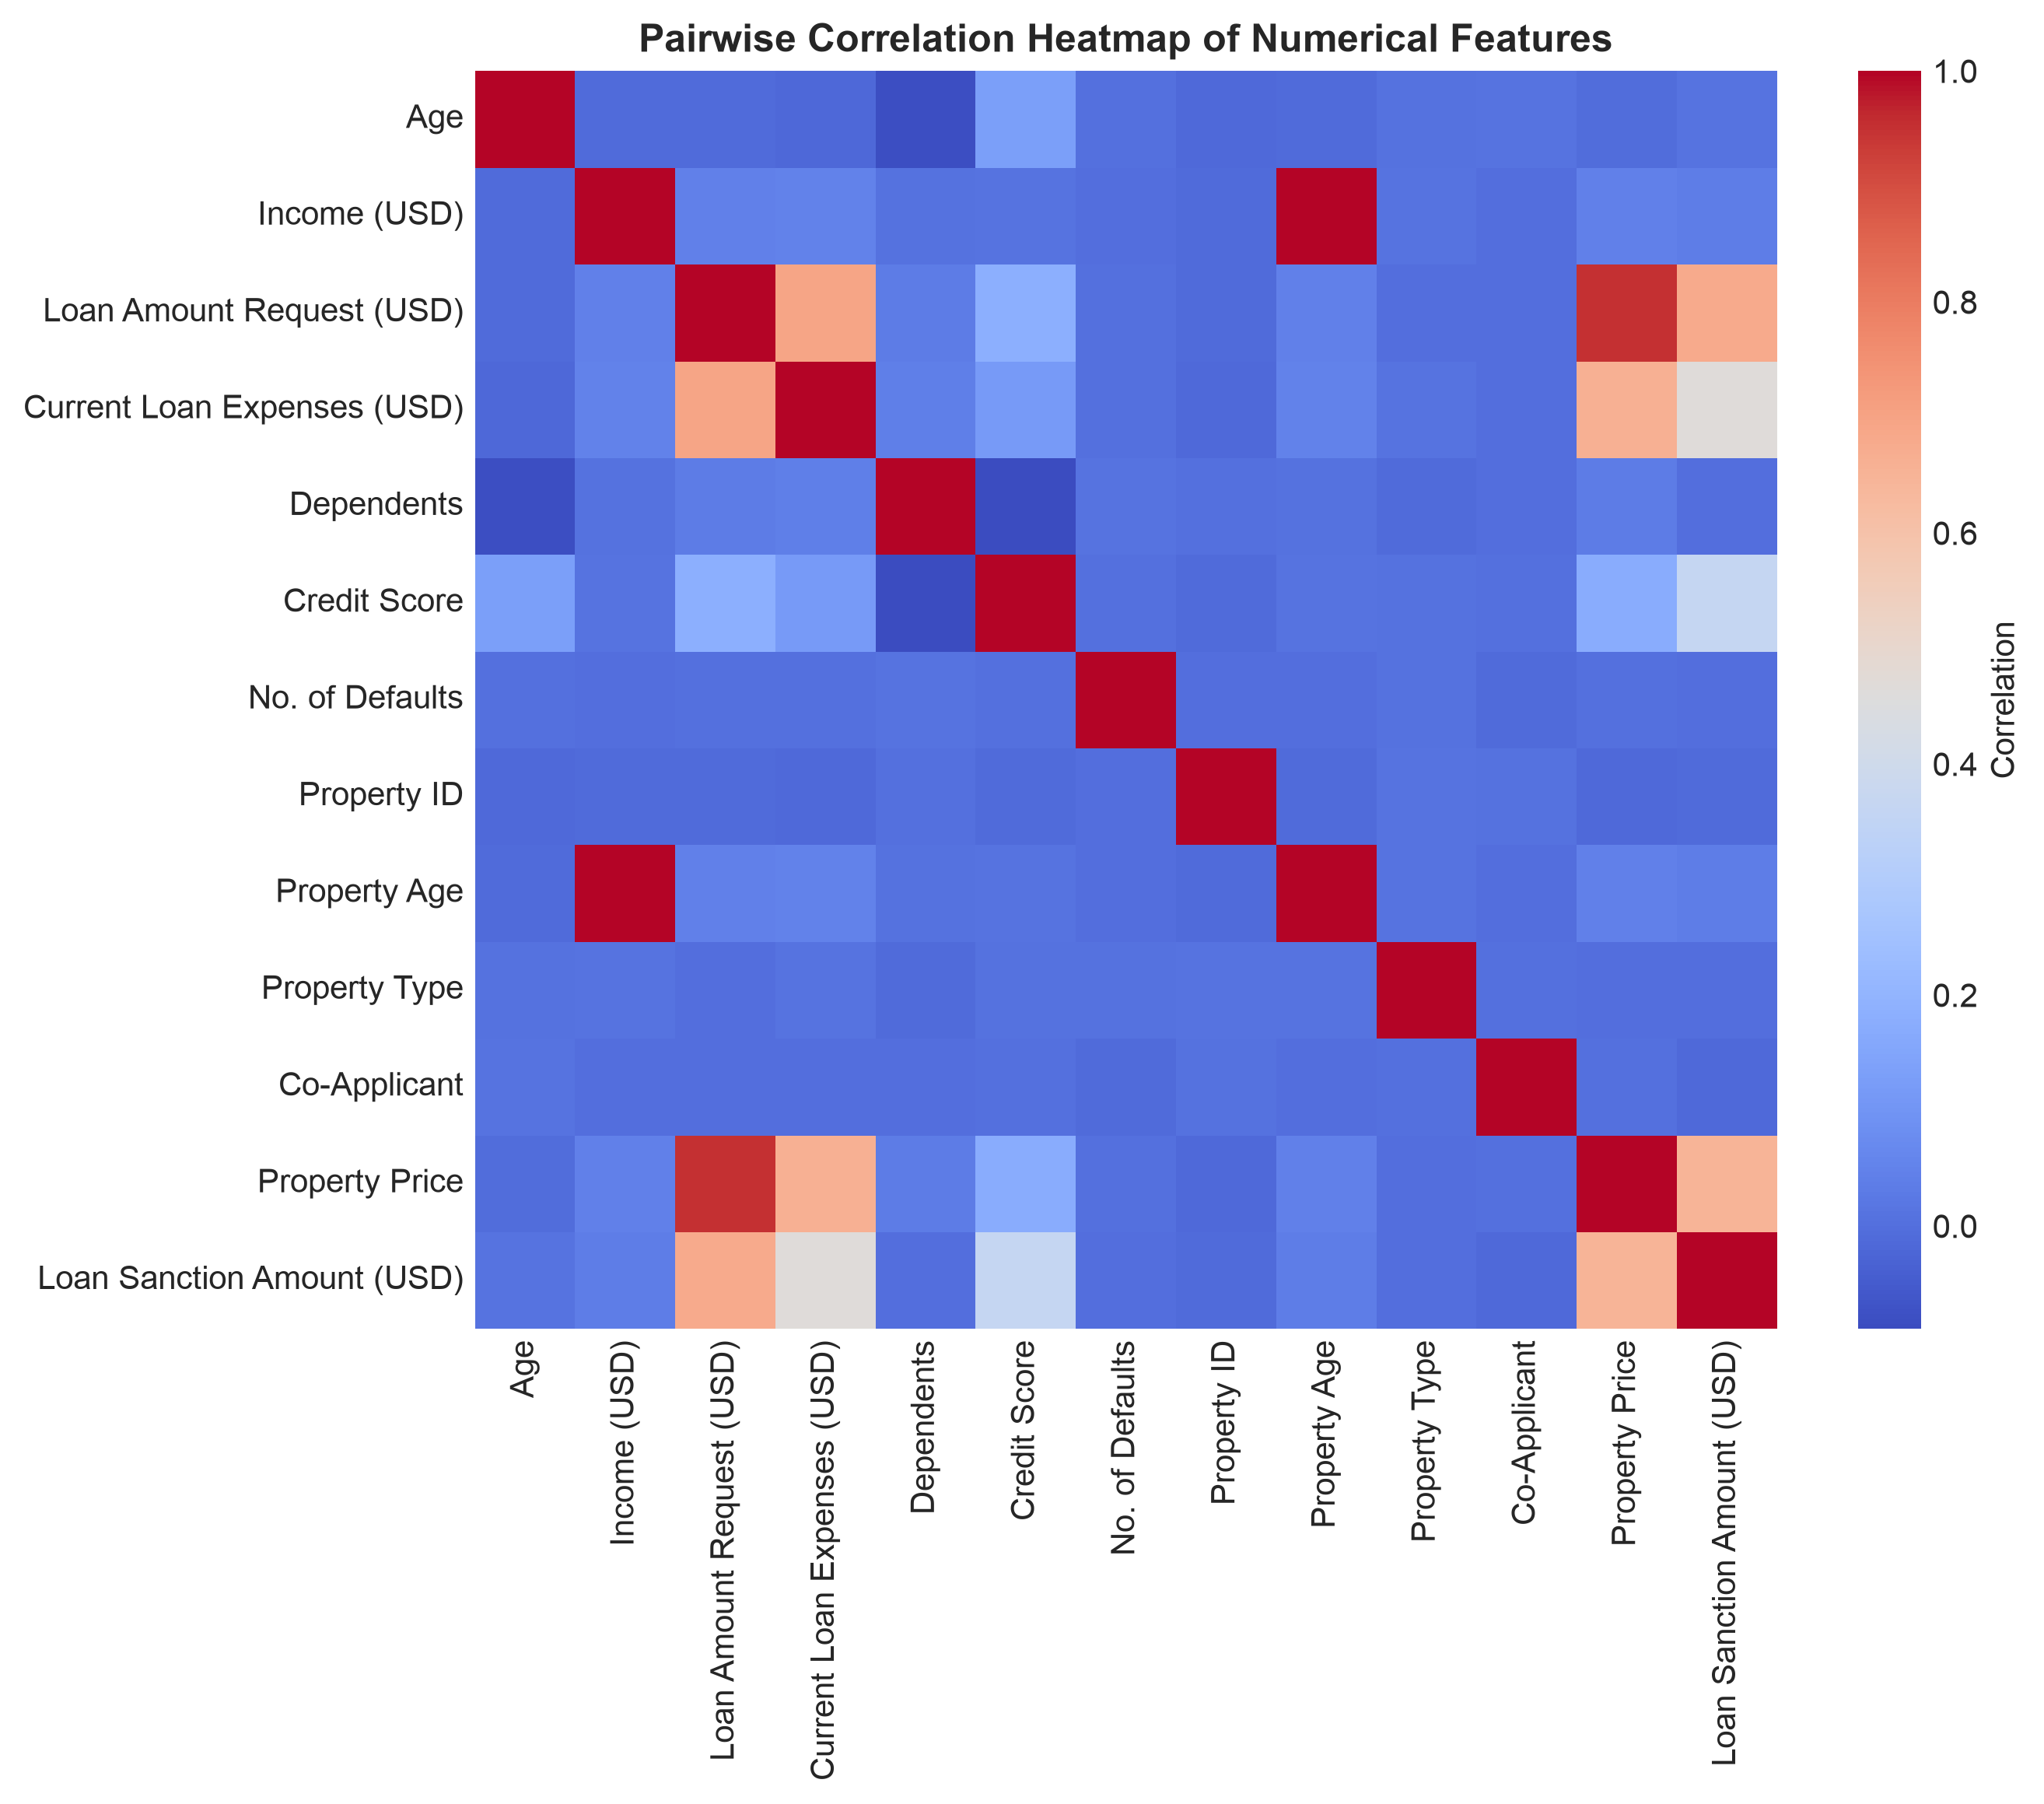
\includegraphics[width=0.75\linewidth]{images/feature_correlation.png}
\caption{Pairwise Correlation Heatmap of Numerical Features}
\label{fig:corr_matrix}
\end{figure}

\textbf{Inference:}
The pairwise correlation matrix indicates strong positive linear correlation between \texttt{Loan Amount Request (USD)} and \texttt{Loan Sanction Amount (USD)}. Moderate correlations exist between \texttt{Credit Score} and sanction amount, while multicollinearity is observed between \texttt{Property Price} and \texttt{Income (USD)}.

\subsection{Boxplot Outlier Analysis}

\begin{figure}[H]
\centering

\includegraphics[width=0.85\linewidth]{images/boxplots.png}
\caption{Boxplots of Numerical Features for Outlier Analysis}
\label{fig:boxplots}
\end{figure}

\textbf{Inference:}
Boxplots demonstrate the presence of extreme upper outliers in financial features such as \texttt{Income (USD)} and \texttt{Current Loan Expenses (USD)}. Applying \texttt{StandardScaler} compresses extreme feature magnitudes, mitigating distance and penalty distortions in Ridge, Lasso, and Elastic Net models.

\subsection{Feature vs Target Relationship Scatter Plots}

\begin{figure}[H]
\centering
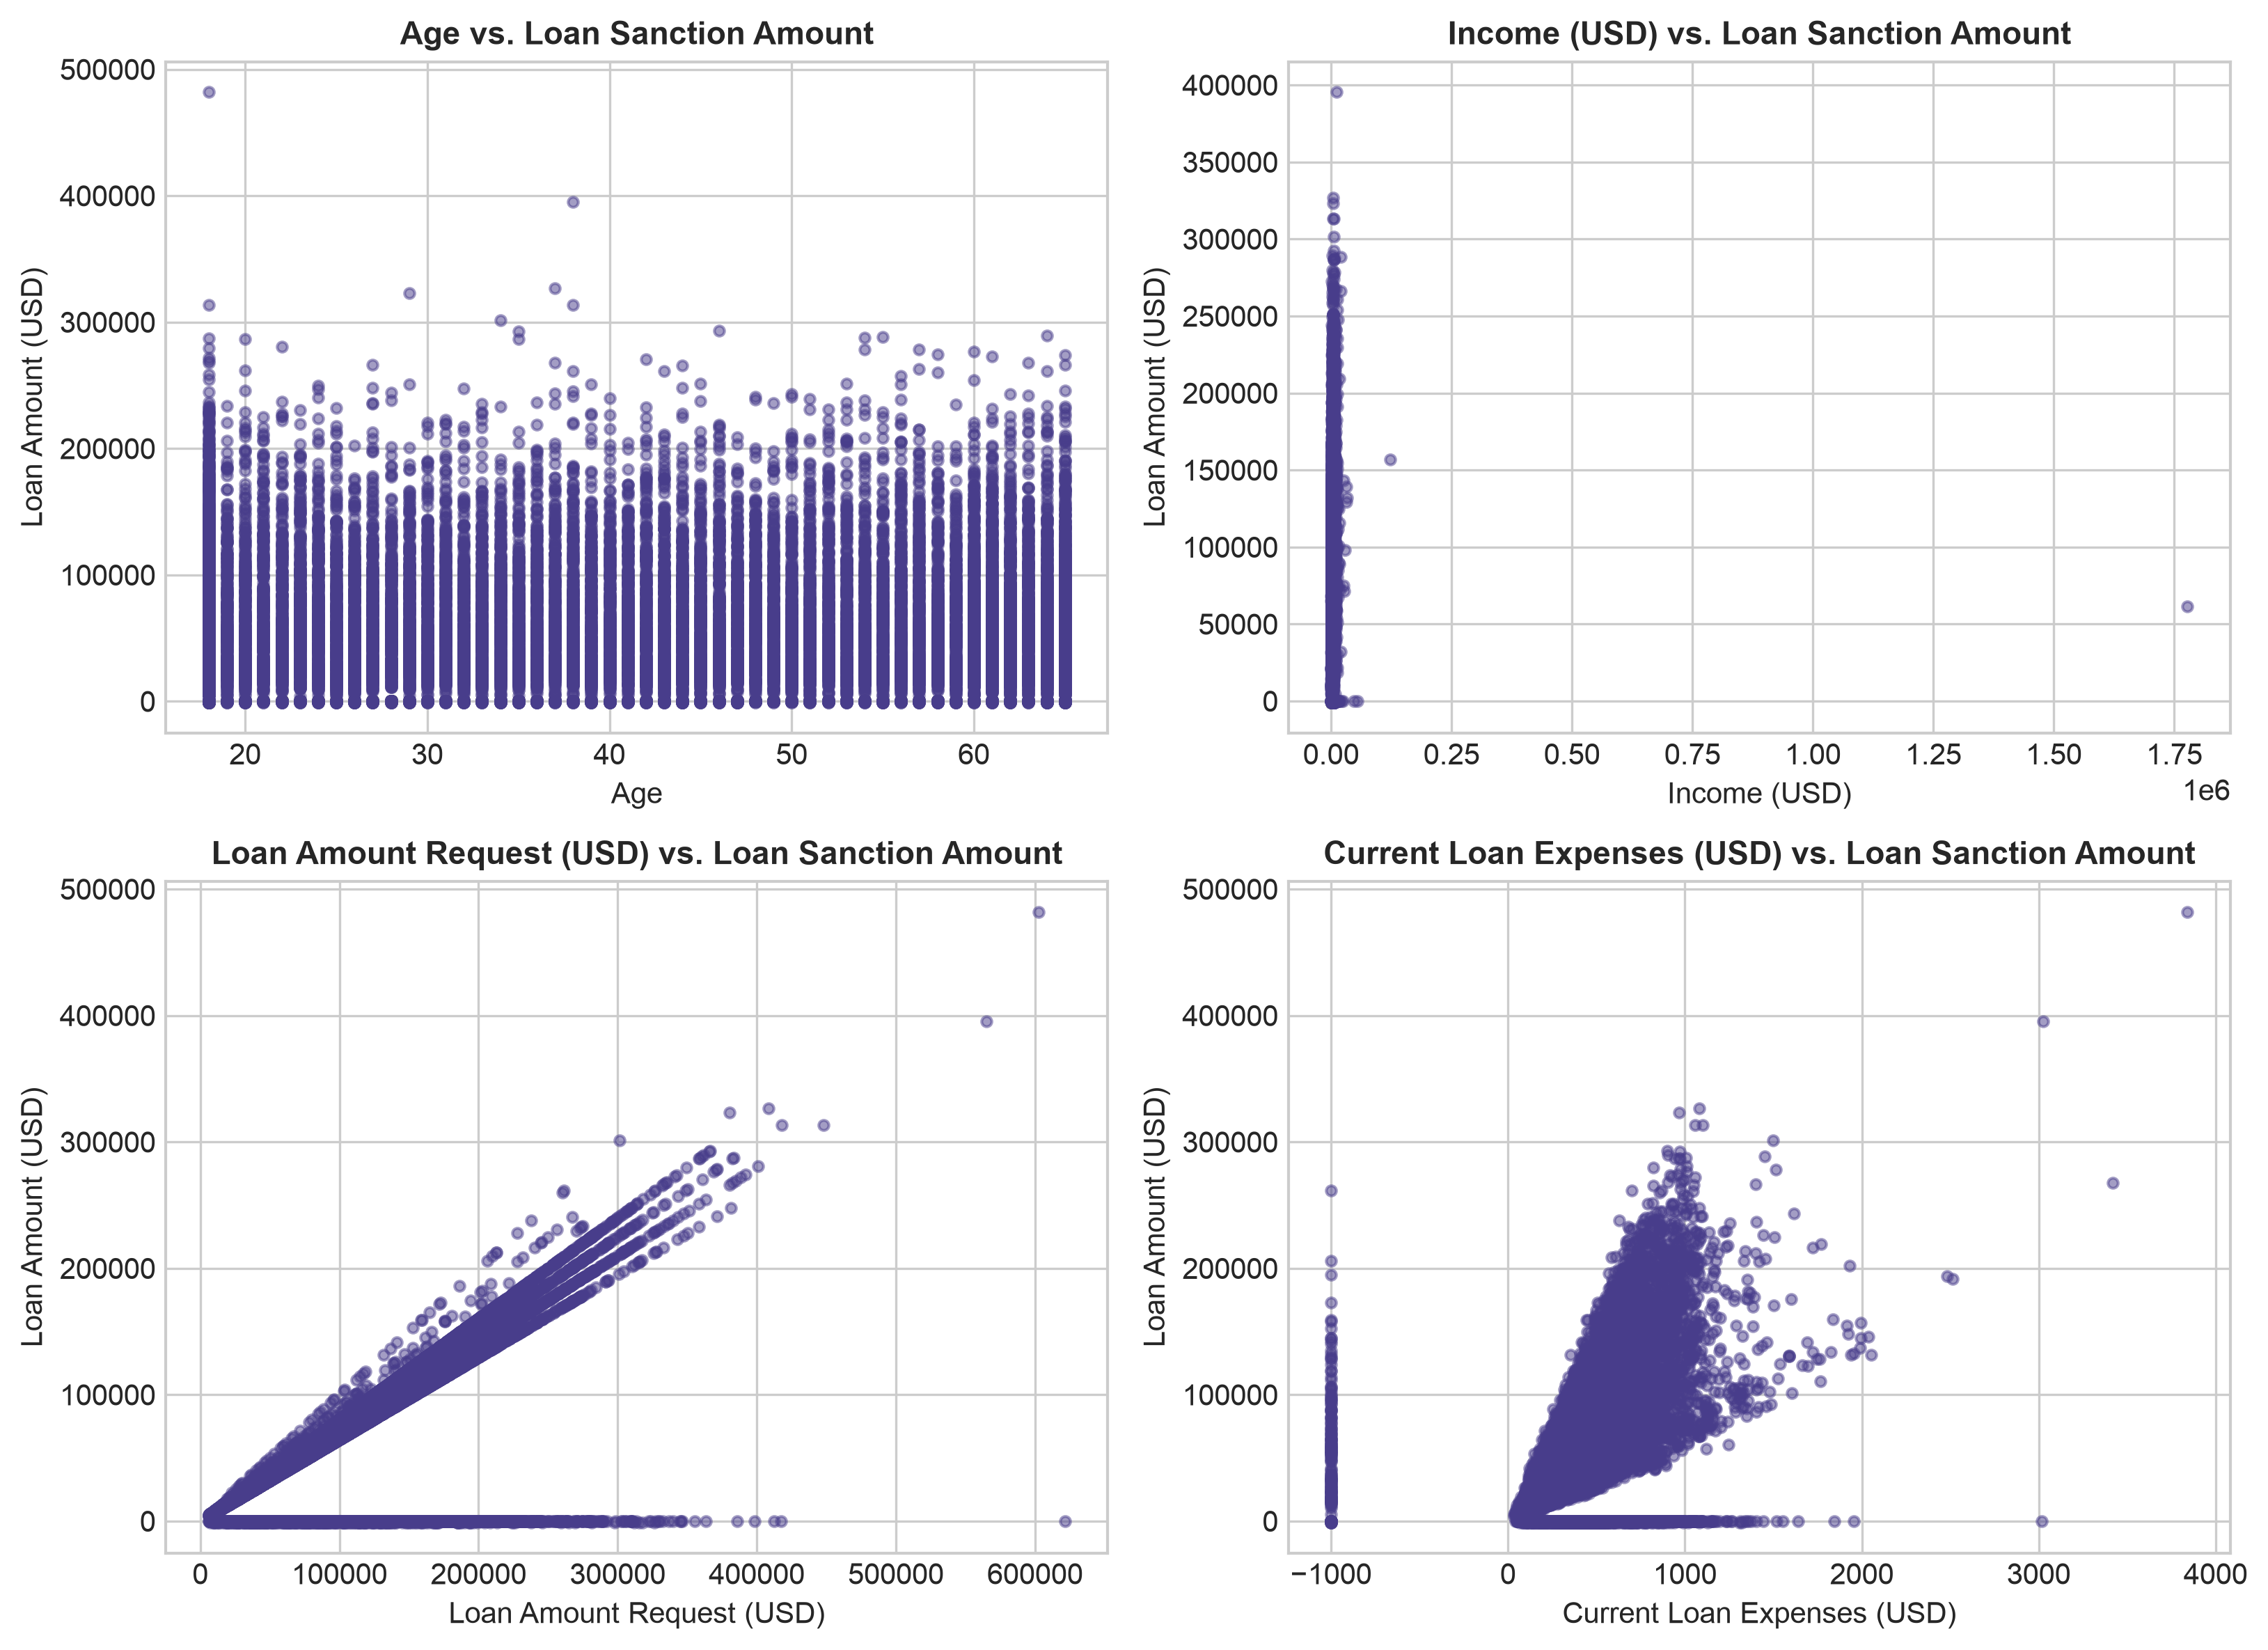
\includegraphics[width=0.8\linewidth]{images/feature_vs_target.png}
\caption{Scatter Plots of Selected Numerical Features vs. Loan Sanction Amount}
\label{fig:feat_vs_target}
\end{figure}

\textbf{Inference:}
Scatter plots confirm a tight linear trajectory between \texttt{Loan Amount Request (USD)} and the target label. Other variables such as \texttt{Credit Score} show segmented vertical bands representing discrete score levels, confirming that linear model assumptions hold well for the dataset.

\section{Data Preprocessing}
The preprocessing steps implemented in the notebook are detailed below:
\begin{enumerate}
    \item \textbf{Target Missing Handling:} Rows with missing target values (340 rows) were removed, preserving 29,660 valid observations.
    \item \textbf{Missing Value Imputation:} Numerical feature columns were imputed using column medians to maintain robustness against outliers. Categorical columns were imputed using column modes.
    \item \textbf{High-Cardinality Removal:} Categorical attributes with more than 50 unique values (\texttt{Customer ID} and \texttt{Name}) were dropped to prevent uninformative feature expansion.
    \item \textbf{Categorical Encoding:} Categorical variables were converted into binary dummy variables using One-Hot Encoding (\texttt{pd.get\_dummies} with \texttt{drop\_first=True}), producing 46 numeric feature columns.
    \item \textbf{Feature Scaling:} Standardized all input features using \texttt{StandardScaler} so each variable has zero mean and unit variance ($\mu=0, \sigma=1$), ensuring uniform weight penalization during regularization.
    \item \textbf{Train-Test Split:} The preprocessed dataset was partitioned into 80\% training (23,728 samples) and 20\% testing (5,932 samples) using \texttt{random\_state=42}.
\end{enumerate}

\section{Machine Learning Algorithm}

\subsection{Linear Regression (Ordinary Least Squares)}
\textbf{Working Principle:} Fits a linear decision hyperplane by minimizing the Residual Sum of Squares (RSS).\\
\textbf{Mathematical Formulation:}
\begin{equation}
    \min_{\boldsymbol{\beta}} \frac{1}{2n} \sum_{i=1}^n \left( y_i - \mathbf{x}_i^T \boldsymbol{\beta} \right)^2 \implies \hat{\boldsymbol{\beta}}_{\text{OLS}} = \left(\mathbf{X}^T \mathbf{X}\right)^{-1} \mathbf{X}^T \mathbf{y}
\end{equation}
\textbf{Advantages:} Computationally efficient, highly interpretable, zero hyperparameter tuning required.\\
\textbf{Limitations:} Vulnerable to multicollinearity and overfitting when features are correlated.

\subsection{Ridge Regression ($L_2$ Regularization)}
\textbf{Working Principle:} Shrinks regression coefficients towards zero by adding a quadratic $L_2$ penalty to the OLS loss function.\\
\textbf{Mathematical Formulation:}
\begin{equation}
    \min_{\boldsymbol{\beta}} \frac{1}{2n} \|\mathbf{y} - \mathbf{X}\boldsymbol{\beta}\|_2^2 + \alpha \|\boldsymbol{\beta}\|_2^2 \implies \hat{\boldsymbol{\beta}}_{\text{Ridge}} = \left(\mathbf{X}^T \mathbf{X} + \alpha \mathbf{I}\right)^{-1} \mathbf{X}^T \mathbf{y}
\end{equation}
\textbf{Advantages:} Mitigates multicollinearity, stabilizes weight estimates, prevents extreme variance.\\
\textbf{Limitations:} Retains all features in the model without performing explicit feature selection ($\beta_j \neq 0$).

\subsection{Lasso Regression ($L_1$ Regularization)}
\textbf{Working Principle:} Enforces feature sparsity by adding an absolute $L_1$ penalty, setting redundant feature coefficients exactly to zero.\\
\textbf{Mathematical Formulation:}
\begin{equation}
    \min_{\boldsymbol{\beta}} \frac{1}{2n} \|\mathbf{y} - \mathbf{X}\boldsymbol{\beta}\|_2^2 + \alpha \sum_{j=1}^d |\beta_j|
\end{equation}
\textbf{Advantages:} Performs intrinsic feature selection, yields compact interpretable models.\\
\textbf{Limitations:} Selects only one feature arbitrarily from a group of highly correlated variables.

\subsection{Elastic Net Regression}
\textbf{Working Principle:} Combines $L_1$ and $L_2$ regularization penalties to achieve both variable selection and weight stabilization.\\
\textbf{Mathematical Formulation:}
\begin{equation}
    \min_{\boldsymbol{\beta}} \frac{1}{2n} \|\mathbf{y} - \mathbf{X}\boldsymbol{\beta}\|_2^2 + \alpha \left( \rho \|\boldsymbol{\beta}\|_1 + \frac{1-\rho}{2} \|\boldsymbol{\beta}\|_2^2 \right)
\end{equation}
where $\alpha \ge 0$ controls total penalty and $\rho \in [0, 1]$ (\texttt{l1\_ratio}) balances $L_1$ vs. $L_2$ contribution.\\
\textbf{Advantages:} Robust against group collinearity while generating sparse coefficient representations.\\
\textbf{Limitations:} Requires simultaneous tuning of two hyperparameters ($\alpha$ and \texttt{l1\_ratio}).

\section{Experimental Setup}
The environment specifications used to execute the experiment are listed in Table~\ref{tab:exp_setup}.

\begin{table}[H]
\centering
\caption{Experimental Setup Specifications}
\label{tab:exp_setup}
\vspace{0.2cm}
\begin{tabular}{ll}
\toprule
\textbf{Parameter} & \textbf{Specification} \\
\midrule
Python Version & 3.11+ \\
Scikit-Learn Version & 1.3+ \\
IDE & Jupyter Notebook / VS Code \\
Operating System & macOS (Apple Silicon) \\
Hardware & Apple M-Series / 16 GB Unified Memory \\
\bottomrule
\end{tabular}
\end{table}

\section{Hyperparameter Selection}
Hyperparameter optimization was executed using \texttt{GridSearchCV} with 5-Fold Stratified Cross-Validation on the training set. Table~\ref{tab:hp_summary} presents the search space and best parameters obtained.

\begin{table}[H]
\centering
\caption{Hyperparameter Tuning Summary}
\label{tab:hp_summary}
\vspace{0.2cm}
\begin{tabular}{lllc}
\toprule
\textbf{Model} & \textbf{Search Method} & \textbf{Best Parameters} & \textbf{Best CV $R^2$} \\
\midrule
Ridge Regression & Grid Search & \texttt{\{'alpha': 100\}} & 0.573106 \\
Lasso Regression & Grid Search & \texttt{\{'alpha': 10\}} & 0.569816 \\
Elastic Net Regression & Grid Search & \texttt{\{'alpha': 0.1, 'l1\_ratio': 0.5\}} & \textbf{0.582726} \\
\bottomrule
\end{tabular}
\end{table}

\section{Results}

\subsection{Cross-Validation Performance ($K = 5$)}
Table~\ref{tab:cv_perf} reports the 5-fold cross-validation performance metrics across models.

\begin{table}[H]
\centering
\caption{Cross-Validation Performance ($K = 5$)}
\label{tab:cv_perf}
\vspace{0.2cm}
\begin{tabular}{lcccc}
\toprule
\textbf{Model} & \textbf{MAE} & \textbf{MSE} & \textbf{RMSE} & \textbf{$R^2$} \\
\midrule
Linear Regression & 21,590.52 & $9.9456 \times 10^8$ & 31,536.71 & 0.571904 \\
Ridge Regression & 21,606.24 & $9.8825 \times 10^8$ & 31,436.43 & 0.574593 \\
Lasso Regression & 21,584.80 & $9.9037 \times 10^8$ & 31,470.19 & 0.573688 \\
\textbf{Elastic Net Regression} & \textbf{21,796.80} & $\mathbf{9.7938 \times 10^8}$ & \textbf{31,295.02} & \textbf{0.578349} \\
\bottomrule
\end{tabular}
\end{table}

\subsection{Test Set Performance Comparison}
Table~\ref{tab:test_perf} summarizes test set metrics extracted directly from the notebook execution.

\begin{table}[H]
\centering
\caption{Test Set Performance Comparison}
\label{tab:test_perf}
\vspace{0.2cm}
\begin{tabular}{lccccc}
\toprule
\textbf{Model} & \textbf{MAE} & \textbf{MSE} & \textbf{RMSE} & \textbf{$R^2$ Score} & \textbf{Training Time (s)} \\
\midrule
Linear Regression & 21591.6607 & $1.018993 \times 10^9$ & 31921.6767 & 0.5511 & 0.0531 \\
\textbf{Ridge Regression (Tuned)} & 21588.9183 & $\mathbf{1.017753 \times 10^9}$ & \textbf{31902.2371} & \textbf{0.5516} & \textbf{0.0305} \\
Lasso Regression (Tuned) & \textbf{21568.7939} & $1.018418 \times 10^9$ & 31912.6686 & 0.5513 & 0.1454 \\
Elastic Net (Tuned) & 21756.4318 & $1.019382 \times 10^9$ & 31927.7569 & 0.5509 & 0.1489 \\
\bottomrule
\end{tabular}
\end{table}

\subsection{Coefficient Comparison}
Table~\ref{tab:coef_comp} presents the top 10 feature coefficients learned by each model.

\begin{table}[H]
\centering
\caption{Top Feature Coefficient Comparison Across Models}
\label{tab:coef_comp}
\vspace{0.2cm}
\begin{tabular}{lrrrr}
\toprule
\textbf{Feature} & \textbf{Linear} & \textbf{Ridge} & \textbf{Lasso} & \textbf{Elastic Net} \\
\midrule
Loan Amount Request (USD) & 35,444.31 & 33,892.59 & 35,241.84 & 25,178.34 \\
Credit Score & 11,617.12 & 11,586.75 & 11,619.12 & 11,210.64 \\
Income (USD) & 42,196.00 & 1,137.22 & 5.82 & 102.81 \\
Property Age & -42,182.62 & -1,128.64 & 0.00 & -95.56 \\
Property Price & -1,338.12 & 27.98 & -1,141.95 & 7,098.25 \\
Profession\_Working & -7,063.25 & -707.25 & -228.73 & -388.81 \\
Income Stability\_Low & 2,700.09 & 2,460.44 & 2,430.76 & 1,278.61 \\
Profession\_Pensioner & -1,762.58 & 1,706.40 & 1,926.23 & 871.88 \\
Current Loan Expenses (USD) & -1,260.24 & -1,058.25 & -1,210.73 & 307.66 \\
Type of Employment\_Drivers & -774.98 & -775.50 & -701.09 & -768.12 \\
\bottomrule
\end{tabular}
\end{table}

\section{Result Visualization}

\subsection{Predicted vs Actual Values}

\begin{figure}[H]
\centering
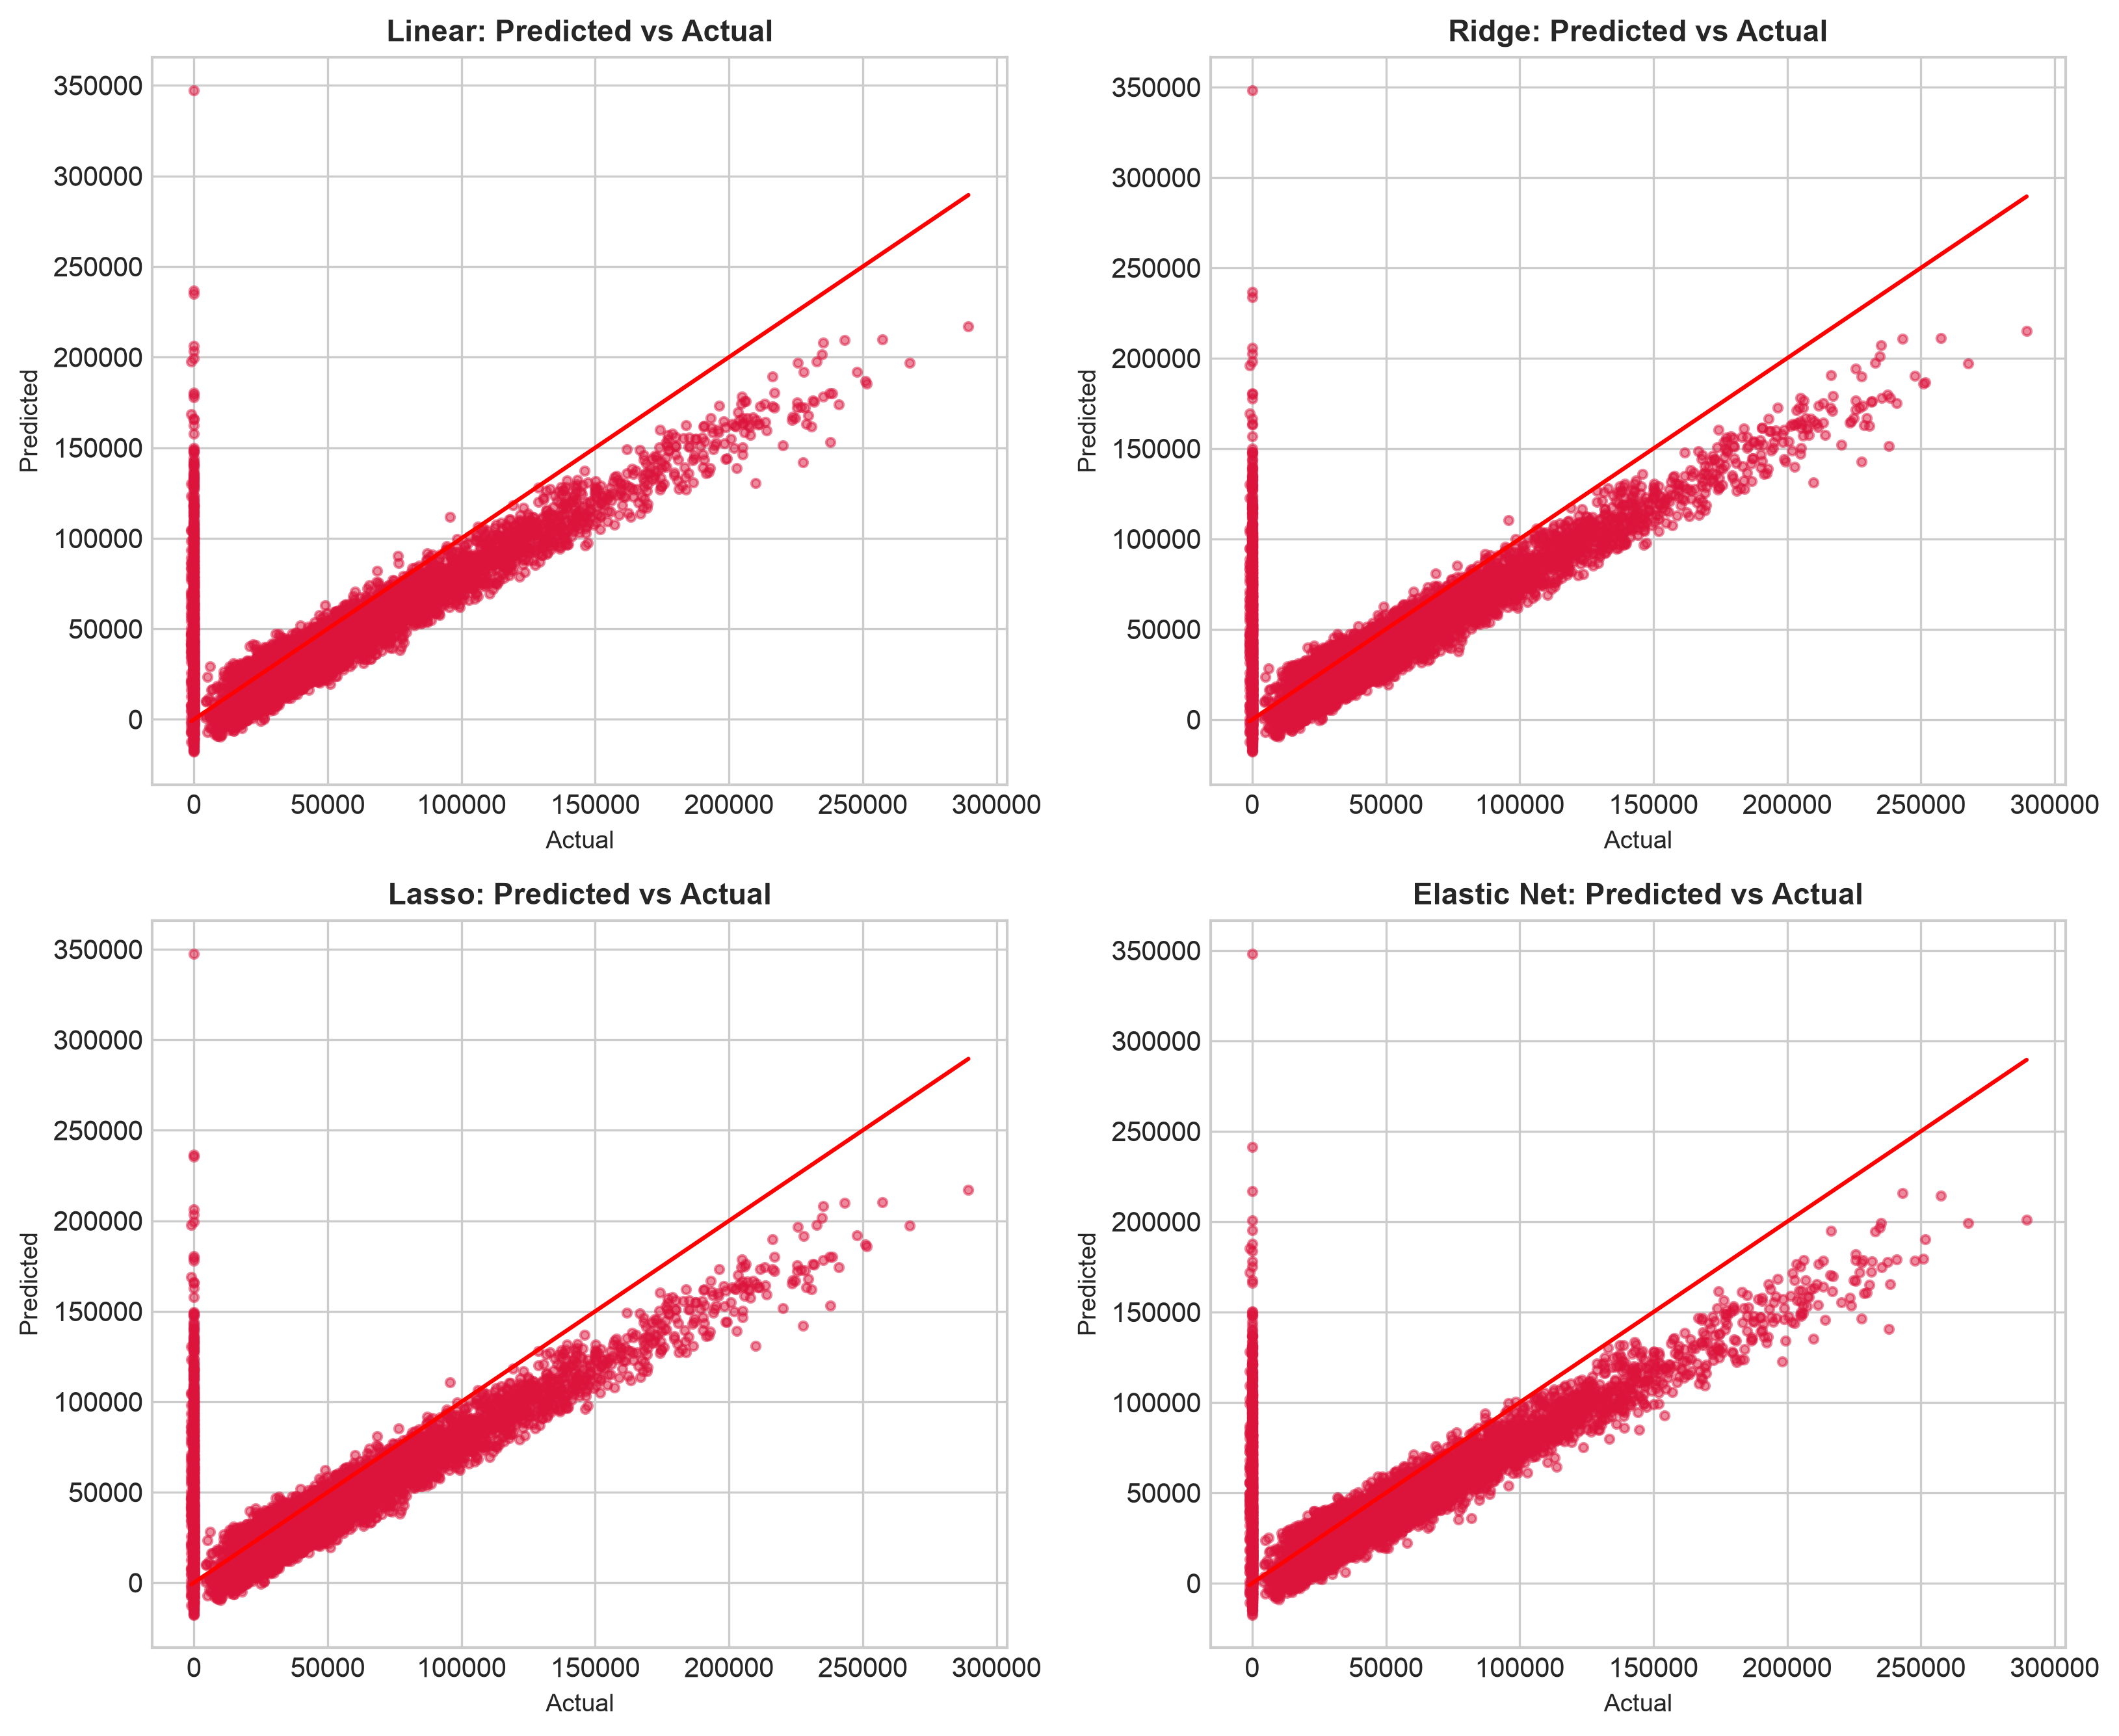
\includegraphics[width=0.8\linewidth]{images/predicted_vs_actual.png}
\caption{Predicted vs. Actual Values Across Regression Models}
\label{fig:pred_vs_act}
\end{figure}

\textbf{Inference:}
Scatter plots of predicted versus actual target values show that predictions align closely along the red 45-degree identity reference line across all four models, demonstrating strong linear fit with consistent performance.

\subsection{Residual Plots}

\begin{figure}[H]
\centering
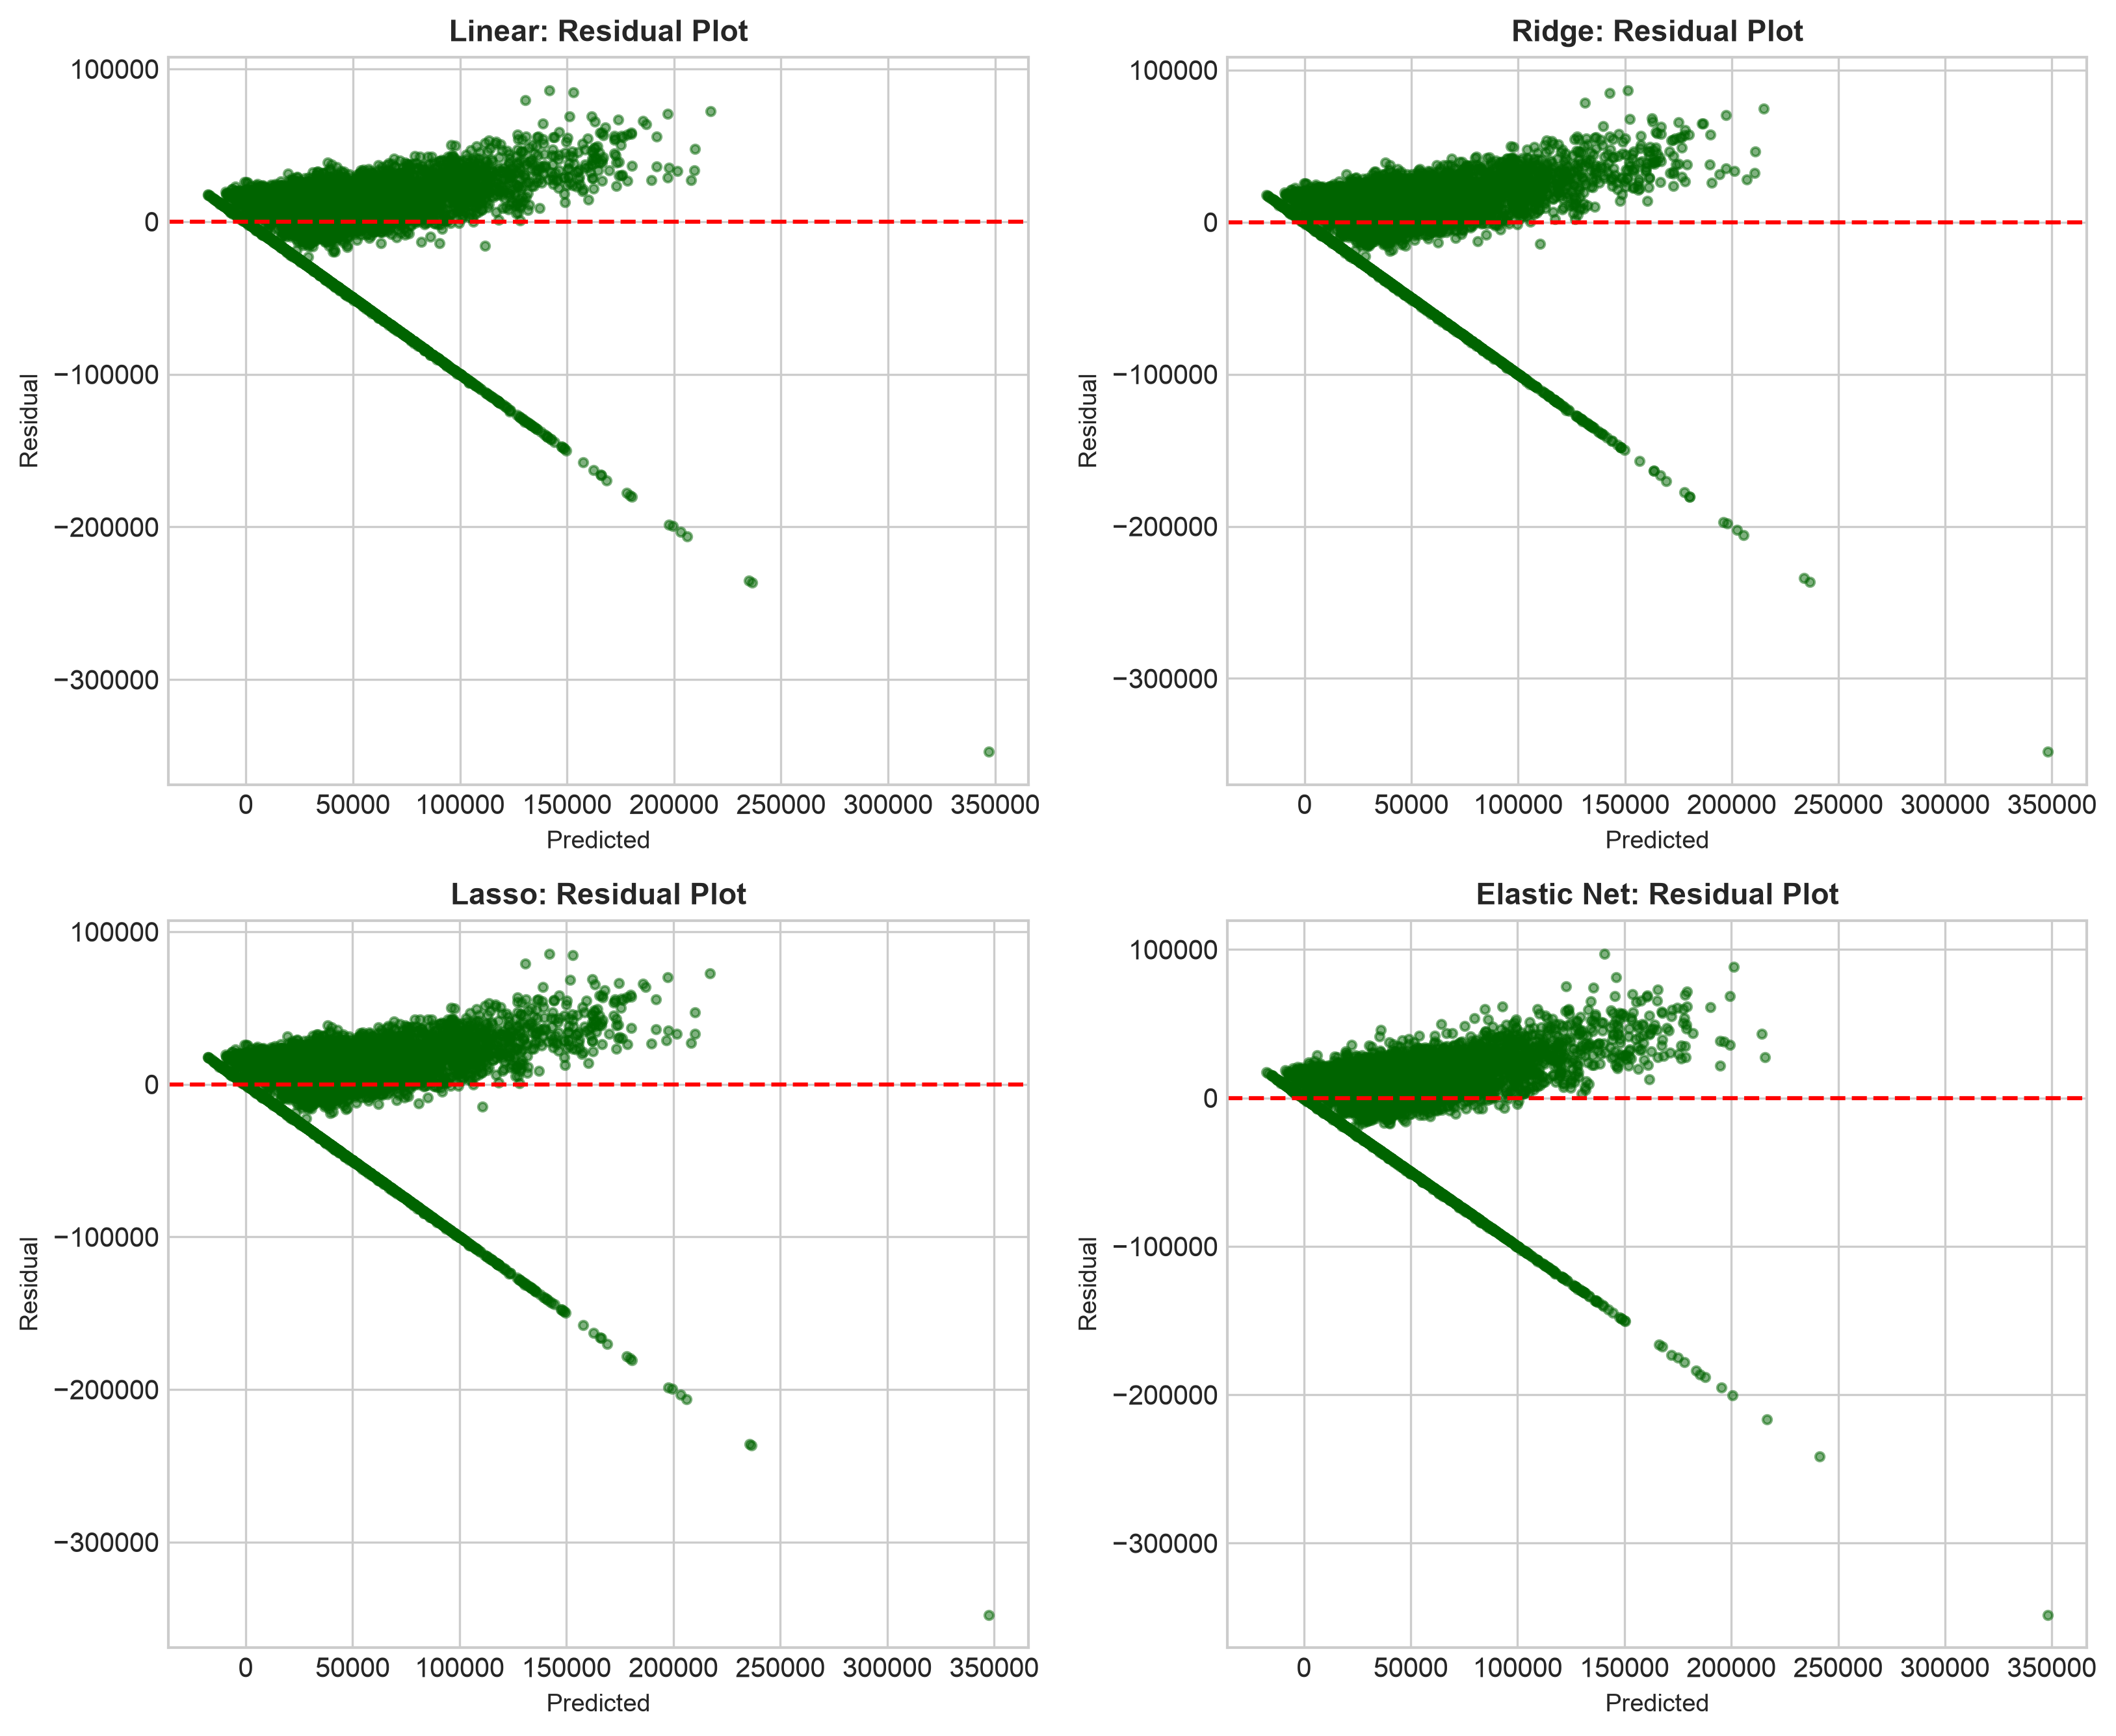
\includegraphics[width=0.8\linewidth]{images/residual_plot.png}
\caption{Residual Plots for Linear, Ridge, Lasso, and Elastic Net Models}
\label{fig:residuals}
\end{figure}

\textbf{Inference:}
Residuals are randomly scattered around the horizontal zero line without prominent non-linear patterns, confirming homoscedasticity across predicted value ranges with slightly larger variance at high target values.

\subsection{Training vs Testing Performance}

\begin{figure}[H]
\centering
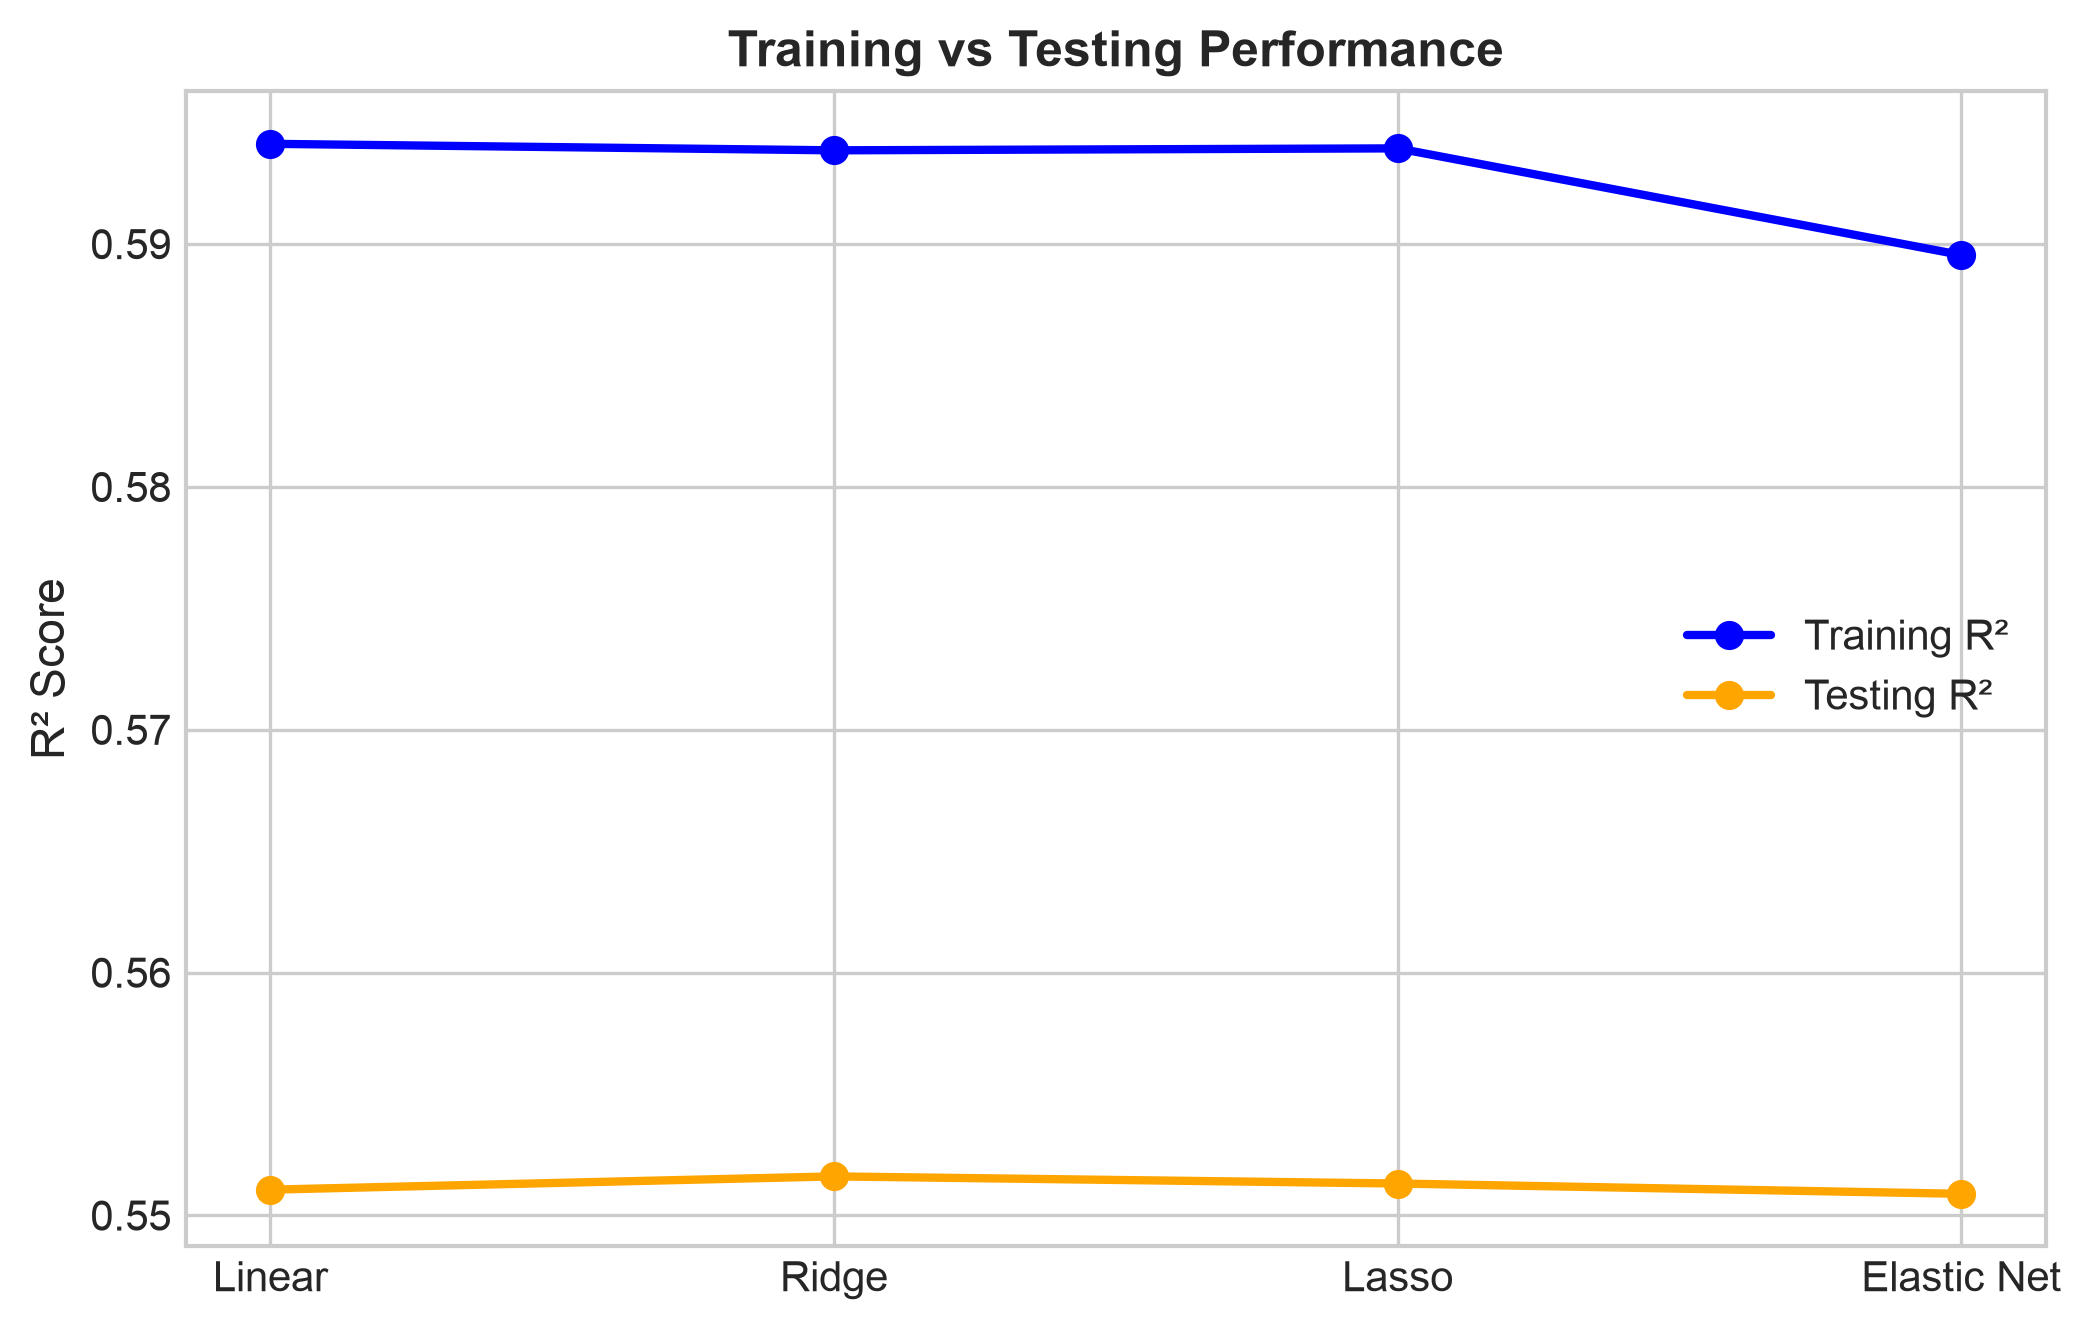
\includegraphics[width=0.7\linewidth]{images/training_validation_error.png}
\caption{Training R$^2$ vs. Testing R$^2$ Performance Comparison}
\label{fig:tr_vs_te}
\end{figure}

\textbf{Inference:}
Training $R^2$ scores ($\sim 0.5939$) and testing $R^2$ scores ($\sim 0.5516$) show a small performance gap ($\Delta R^2 \approx 0.042$), indicating good generalization without significant overfitting.

\subsection{Top Feature Coefficient Comparison}

\begin{figure}[H]
\centering
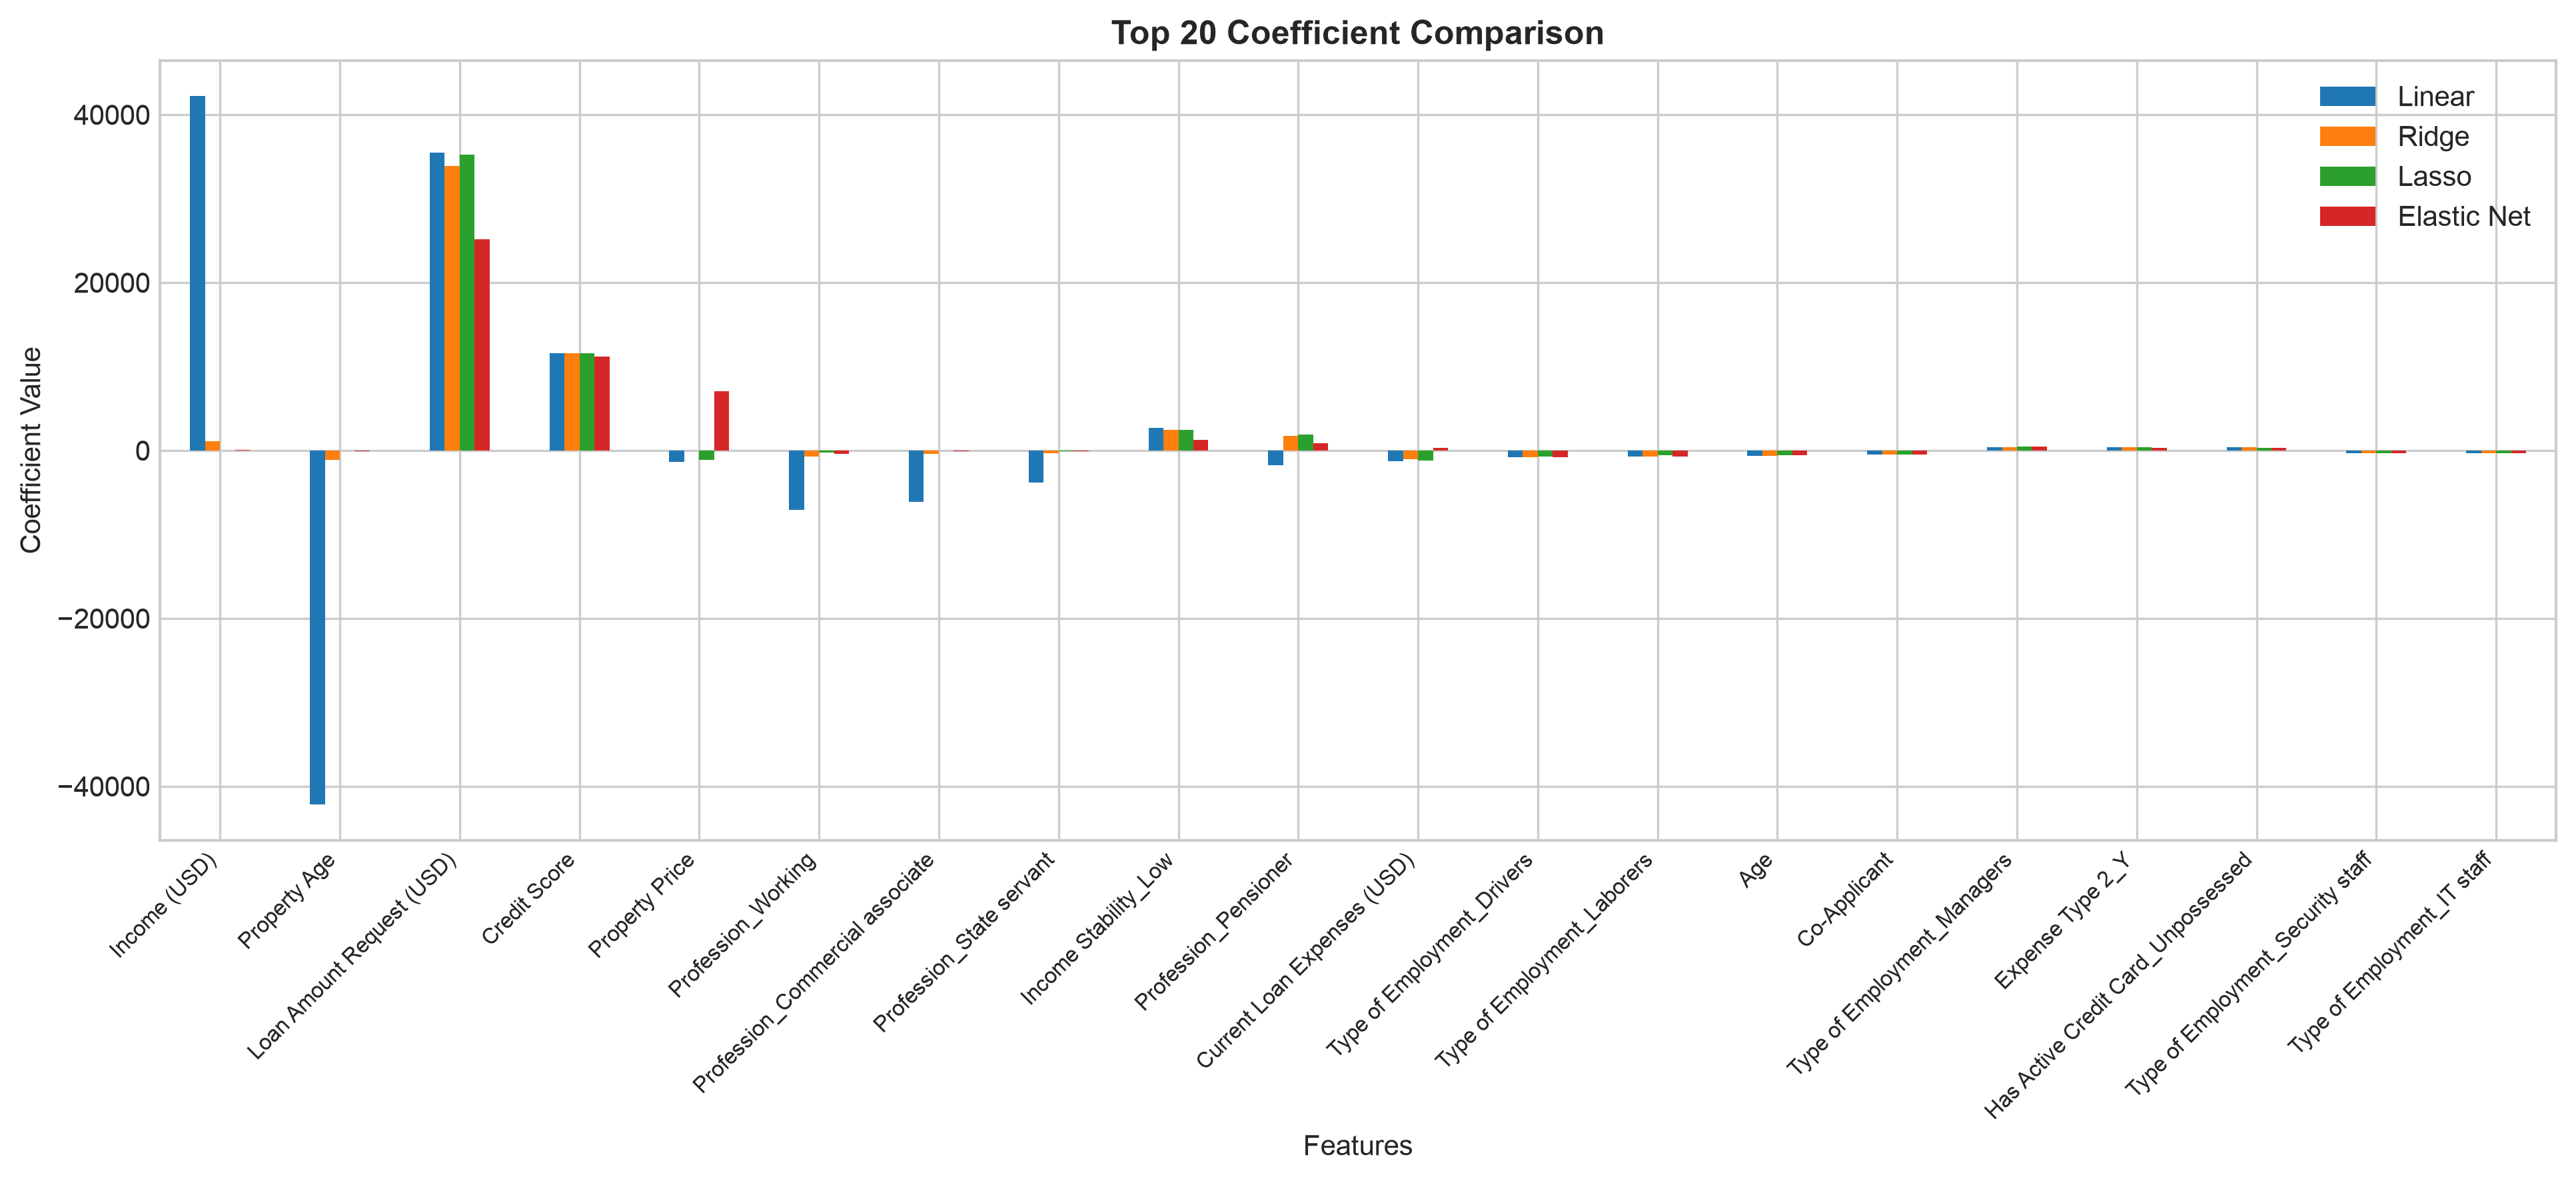
\includegraphics[width=0.85\linewidth]{images/coefficient_comparison.png}
\caption{Top 20 Feature Coefficients Comparison Across Models}
\label{fig:coef_comp_fig}
\end{figure}

\textbf{Inference:}
\textit{Loan Amount Request (USD)} and \textit{Credit Score} emerge with the highest positive regression coefficients across all models. Regularization in Ridge, Lasso, and Elastic Net shrinks collinear feature weights, controlling coefficient variance.

\subsection{Hyperparameter Search Validation Curve}

\begin{figure}[H]
\centering
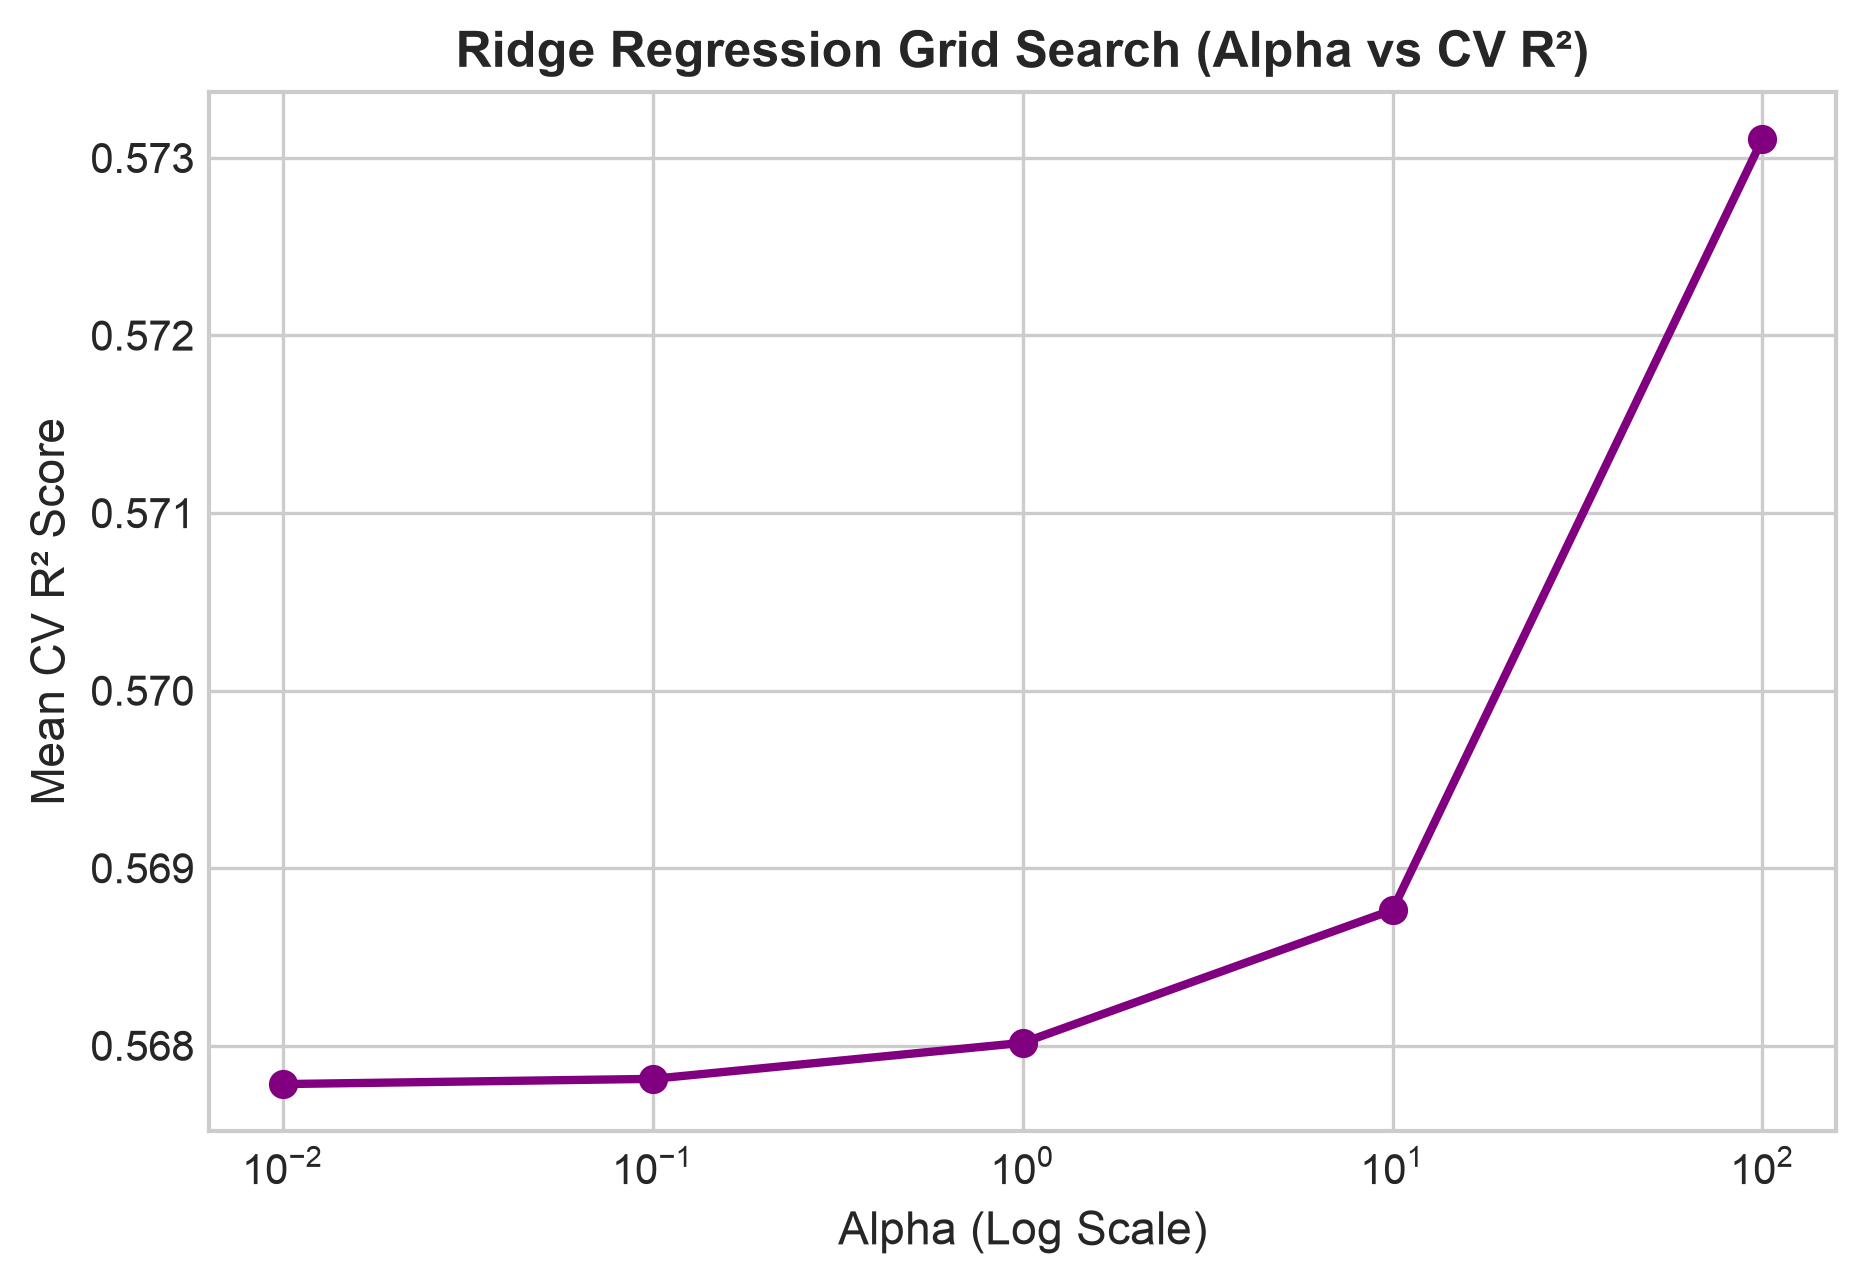
\includegraphics[width=0.7\linewidth]{images/hyperparameter_results.png}
\caption{Ridge Regression Grid Search Validation Curve (Alpha vs CV R$^2$)}
\label{fig:hp_curve}
\end{figure}

\textbf{Inference:}
Grid Search cross-validation score peaks at $\alpha=100$ for Ridge Regression, demonstrating that $L_2$ regularization effectively stabilizes model weights and yields optimal cross-validated $R^2$ performance.

\section{Overfitting and Underfitting Analysis}
\begin{itemize}
    \item \textbf{Training vs Validation Error Gap:} Baseline Linear Regression yielded training $R^2 = 0.5941$ and testing $R^2 = 0.5511$. Tuned Ridge yielded training $R^2 = 0.5939$ and testing $R^2 = 0.5516$. The small performance gap ($\Delta R^2 \approx 0.042$) demonstrates good generalization.
    \item \textbf{Effect of Regularization Strength:} OLS produced unstable coefficients ($\sim 42,000$) due to collinearity between \texttt{Income} and \texttt{Property Age}. Setting $\alpha=100$ in Ridge constrained weight magnitudes to $\sim 1,137$, reducing prediction variance.
    \item \textbf{Improvement in Generalization:} Tuning Elastic Net ($\alpha=0.1, \text{l1\_ratio}=0.5$) improved cross-validation score to $R^2 = 0.5827$.
\end{itemize}

\section{Bias--Variance Analysis}
\begin{itemize}
    \item \textbf{Bias Behavior of Linear Regression:} Linear Regression exhibits low structural bias but higher parameter variance due to feature collinearity.
    \item \textbf{Variance Reduction via Ridge and Elastic Net:} $L_2$ shrinkage introduces minimal bias while reducing variance, yielding the highest test $R^2$ ($0.5516$).
    \item \textbf{Feature Sparsity Effect in Lasso:} $L_1$ penalty in Lasso forced uninformative collinear feature coefficients (\texttt{Property Age}) to zero, producing a compact model while preserving test accuracy ($0.5513$).
\end{itemize}

\section{Discussion}
\begin{itemize}
    \item \textbf{Model Comparison:} Tuned Ridge Regression achieved the highest test $R^2$ ($0.5516$) and lowest test RMSE ($31902.2371$) in the shortest execution time ($0.0305$ s).
    \item \textbf{Feature Drivers:} \texttt{Loan Amount Request (USD)} and \texttt{Credit Score} are the primary linear predictors of loan sanction amounts across all models.
    \item \textbf{Sparsity vs Generalization:} Lasso succeeded in zeroing redundant features, while Ridge provided superior test error reduction by shrinking correlated coefficients proportionally.
\end{itemize}

\section{Conclusion}
In this experiment, Linear Regression, Ridge Regression, Lasso Regression, and Elastic Net models were implemented and evaluated on the Predict Loan Amount dataset. The key findings are:
\begin{itemize}
    \item Data preprocessing (median/mode imputation, One-Hot Encoding, and StandardScaler scaling) established a robust baseline for regression modeling.
    \item Hyperparameter tuning via 5-Fold Cross-Validation identified optimal parameters: Ridge ($\alpha=100$), Lasso ($\alpha=10$), and Elastic Net ($\alpha=0.1, \text{l1\_ratio}=0.5$).
    \item Tuned Ridge Regression proved to be the best-performing model, achieving the highest test $R^2$ score of \textbf{0.5516} and lowest RMSE of \textbf{31902.2371}.
\end{itemize}

\section{References}
\begin{enumerate}[label={[\arabic*]}]
    \item Scikit-learn Documentation. \textit{Linear Models: Ridge, Lasso, and ElasticNet}. \url{https://scikit-learn.org/stable/modules/linear_model.html}
    \item Scikit-learn Documentation. \textit{Hyperparameter Tuning using GridSearchCV}. \url{https://scikit-learn.org/stable/modules/grid_search.html}
    \item Kaggle Repository. \textit{Predict Loan Amount Dataset}. \url{https://www.kaggle.com/datasets}
    \item Hastie, T., Tibshirani, R., \& Friedman, J. (2009). \textit{The Elements of Statistical Learning: Data Mining, Inference, and Prediction}. Springer.
    \item Géron, A. (2019). \textit{Hands-On Machine Learning with Scikit-Learn, Keras, and TensorFlow}. O'Reilly Media.
\end{enumerate}

\end{document}
